\documentclass[a4paper,11pt,oneside]{book}
% =====================================================================
% de_style.tex: Differential Equations (Ch11) homework / test layout.
% = Ch10 di_style (copied as de_core.tex; header text changed) + the DE
% notation and the framed solution boxes of the v1 DE documents
% (soln / spart, used by the Test worked solutions).
% =====================================================================
% =====================================================================
% di_style.tex: Differential Equations homework / test layout.
% Loads the house preamble (local copies of the AoI worksheet files:
% ws_preamble_build.tex, ws_preamble_local.tex -> ws_figstyles.tex),
% then adds the homework layout used by HW1-HW3 and the Test.
% Usage (before \begin{document}):  \ditle{Homework 1}
% =====================================================================
\input{ws_preamble_build}
\input{ws_preamble_local}
\input{prelim_fonts}% Times New Roman + MathType-style maths (as the prelim papers)
\usepackage{needspace}
\usepackage{zref-savepos,zref-abspage}\makeatletter\zref@addprop{savepos}{abspage}\makeatother
\usepackage{array}

% ---- shortlist toggle ------------------------------------------------
% \ifshortlist true  -> only the questions in SHORTLIST.md (+ challenges)
% A wrapper file sets it with \def\setshortlist{1} before \input-ing the
% main file; the main file can also be edited to say \shortlisttrue.
\newif\ifshortlist
% Task 5: the FINAL homework (= former shortlist) is the default build. HWn.tex -> HWn.pdf.
% A wrapper that sets \def\setfull{1} builds the archive with all original questions.
\ifdefined\setfull\else\shortlisttrue\fi

\makeatletter
% ---- REVIEW build: highlight amended content ---------------------------
% A wrapper sets \def\setreview{1}. In review mode amended text is shaded
% yellow and carries a hover note (PDF tooltip / sticky note); otherwise the
% macros print the content plainly.
%   \chg{note}{inline content}        short inline change (no line breaks), text mode
%   \chgm{note}{math}                 the same inside math mode
%   \begin{chgblock}{note} ... \end{chgblock}   paragraph/display-level change
\newif\ifreview
\ifdefined\setreview \reviewtrue \fi
% hover notes are raw PDF annotations (xdvipdfmx \special; no extra packages).
% Keep notes plain ASCII; balanced parentheses are fine.
\newsavebox{\chg@box}
\newcommand{\chg@ann}[4]{% width, height, depth, note -> invisible markup annotation with a hover note
  \special{pdf:ann width #1 height #2 depth #3 << /Type /Annot /Subtype /Square /Border [0 0 0] /BS << /W 0 >> /C [1 0.85 0] /CA 0.01
    /T (Review) /Subj (Amendment) /Contents (#4) >>}}
\newcommand{\chg@sticky}[1]{\special{pdf:ann width 12pt height 12pt depth 0pt << /Type /Annot /Subtype /Text /Name /Comment
    /C [1 0.85 0] /T (Review) /Subj (Amendment) /Contents (#1) >>}}
\newcommand{\chg}[2]{\ifreview\sbox\chg@box{\colorbox{yellow!60}{#2}}%
  \leavevmode\rlap{\chg@ann{\the\wd\chg@box}{\the\ht\chg@box}{\the\dp\chg@box}{#1}}\usebox\chg@box\else#2\fi}
% \chgm{note}{math}: the same, for use INSIDE math mode (display style kept)
\newcommand{\chgm}[2]{\ifreview\mathchoice{\chg{#1}{$\displaystyle#2$}}{\chg{#1}{$\textstyle#2$}}{\chg{#1}{$\scriptstyle#2$}}{\chg{#1}{$\scriptscriptstyle#2$}}\else#2\fi}
\newtcolorbox{chgbox}[1]{enhanced, breakable, colback=yellow!35, colframe=yellow!35, boxrule=0pt, sharp corners,
  left=2pt, right=14pt, top=1pt, bottom=1pt, before skip=2pt, after skip=2pt,
  overlay first and middle={}, overlay last={}, overlay unbroken and first={\node[anchor=north east, inner sep=1pt] at (frame.north east) {\chg@sticky{#1}\hbox to 12pt{\vrule width 0pt height 12pt}};}}
% \chgnote{note}: just the sticky-note icon (e.g. inside a figure); nothing outside review mode
\newcommand{\chgnote}[1]{\ifreview\chg@sticky{#1}\hbox to 12pt{\vrule width 0pt height 12pt}\fi}
\newenvironment{chgblock}[1]{\ifreview\begin{chgbox}{#1}\fi}{\ifreview\end{chgbox}\fi}

% ---- header ---------------------------------------------------------
\newcommand\di@title{}
\makeatletter
\newcommand{\ditle}[1]{\gdef\di@title{#1}}
\fancypagestyle{di}{\fancyhf{}%
  \lhead{\small \di@title}%
  \rhead{\small Compiled by Maximus Pung Jun}%
  \cfoot{\small\thepage}%
  \renewcommand{\headrulewidth}{0.4pt}}
\pagestyle{di}
% title block on page 1, as in his Typst sheets
\newcommand{\dititleblock}[1][]{\thispagestyle{di}%
  {\LARGE\scshape \di@title}\par\smallskip
  {Compiled by Maximus Pung Jun}\par\ifx&#1&\else\smallskip{\small\textcolor{black!60}{#1}}\par\fi\medskip}
\makeatother
\newcommand{\disection}[1]{\par\bigskip\noindent{\Large\scshape #1}\par\medskip}

% ---- questions --------------------------------------------------------
% \Qhead{label}{source tag}: question heading, tag in brackets on the right
\newcommand{\Qhead}[2]{\par\needspace{8\baselineskip}\bigskip\noindent
  {\large\bfseries #1}\hfill{\small\textcolor{black!60}{[#2]}}\par\smallskip}
% part lists with bold labels as he writes them: \pt{(a)}, \pt{(i)}, \pt{(b) (i)}
\newenvironment{qparts}[1][2.4em]{\begin{list}{}{\setlength\leftmargin{#1}%
  \setlength\labelwidth{\dimexpr#1-0.5em\relax}\setlength\labelsep{0.5em}%
  \setlength\itemsep{0.8ex}\setlength\topsep{0.6ex}\setlength\parsep{0.6ex}%
  \renewcommand\makelabel[1]{\textbf{##1}\hfil}}}{\end{list}}
\newcommand{\pt}[1]{\item[#1]}
% thin horizontal label for a challenge question
\newcommand{\challengebanner}{\par\bigskip\noindent\textcolor{black!50}{\rule[0.5ex]{\linewidth}{0.4pt}}\par
  \noindent{\large\scshape Challenge (optional)}\par}
% upright "units"
\newcommand{\units}[1]{\ \text{units}^{#1}}
% END line
\newcommand{\diend}[1][END OF WORKSHEET]{\par\vspace{2\baselineskip}\begin{center}\textbf{#1}\end{center}}

% ---- question registry (full / shortlist from one source) -------------
% \defQ{n}{tag}{body}   question n of the original sheet
% \defA{n}{answer body} its final answer, as printed in his answer section
% \putQ{n} / \putC{n}   print question n as the next (challenge) question
% \putA{n}              print its answer under the same new label
\newcounter{diq}
\makeatletter
\newcommand{\defQ}[3]{\expandafter\gdef\csname diQtag@#1\endcsname{#2}%
  \expandafter\long\expandafter\gdef\csname diQbody@#1\endcsname{#3}}
\newcommand{\defA}[2]{\expandafter\long\expandafter\gdef\csname diA@#1\endcsname{#2}}
\newcommand{\di@tag}[1]{\csname diQtag@#1\endcsname}% source tag only (no original Q number)
% A question never breaks across pages: it is measured and starts on a new page unless it
% fits whole on the rest of this one (only a question taller than a page may break, and then
% only between parts). Page positions of its start/end (zref labels q-s<n>/q-e<n> in the .aux)
% let the checker verify this.
\newsavebox{\di@qmeas}
\newcommand{\di@placeQ}[1]{\par\setbox\di@qmeas=\vbox{#1}%
  \ifdim\dimexpr\ht\di@qmeas+\dp\di@qmeas\relax<0.95\textheight
    \needspace{\dimexpr\ht\di@qmeas+\dp\di@qmeas+\bigskipamount\relax}\else\needspace{14\baselineskip}\fi
  \zsavepos{q-s\thediq}#1\par\zsavepos{q-e\thediq}}
\newcommand{\putQ}[1]{\stepcounter{diq}%
  \expandafter\xdef\csname diLab@#1\endcsname{\thediq}%
  \di@placeQ{\Qhead{\thediq}{\di@tag{#1}}\csname diQbody@#1\endcsname\par}}
\newcommand{\putC}[1]{\stepcounter{diq}%
  \expandafter\xdef\csname diLab@#1\endcsname{\thediq}%
  \expandafter\gdef\csname diChal@#1\endcsname{1}%
  \di@placeQ{\Qhead{\thediq\quad\normalsize\mdseries\scshape Challenge}{\di@tag{#1}}\csname diQbody@#1\endcsname\par}}
\newcommand{\putA}[1]{\par\needspace{4\baselineskip}%
  \begin{qparts}[2.4em]\item[{\csname diLab@#1\endcsname}]\csname diA@#1\endcsname\end{qparts}\medskip}
% ---- worked solutions: \defS{n}{body}, \putQS{n} prints question n + its solution ----
\newcommand{\defS}[2]{\expandafter\long\expandafter\gdef\csname diS@#1\endcsname{#2}}
\newcommand{\disolhead}{\par\medskip\noindent{\bfseries Solution}\par\nobreak\vspace{-0.6ex}\noindent\textcolor{black!35}{\rule{\linewidth}{0.4pt}}\par\nobreak}
\newcommand{\putQS}[1]{\putQ{#1}\disolhead\csname diS@#1\endcsname\par}
% source of a worked solution; visible only in REVIEW builds. #1: his / pub / pip
\newcommand{\solsrc}[2]{\ifreview\par\noindent\def\di@a{#1}\def\di@b{pip}%
  \ifx\di@a\di@b\colorbox{yellow!60}{\parbox{\dimexpr\linewidth-2\fboxsep-14pt}{\small\textbf{Pip-worked:} #2}}\chgnote{Pip-worked solution. No worked solution by the teacher and no published solution was found. Please check it.}%
  \else{\small\textcolor{black!55}{Source of this solution: #2}}\fi\par\smallskip\fi}
\makeatother
% compact sketch for worked solutions: \solfig[axis options]{plot commands}
\newcommand{\solfig}[2][]{\par\begin{center}\begin{tikzpicture}\begin{axis}[qfig, width=6.6cm, height=5cm, #1]#2\end{axis}\end{tikzpicture}\end{center}}
% a sketch added to an existing worked solution (teacher rule), shaded in REVIEW
\newenvironment{addedsketch}{\begin{chgblock}{Sketch added: teacher rule - every area or volume solution has a sketch.}}{\end{chgblock}}
% answer part list (compact)
\newenvironment{aparts}[1][2.4em]{\begin{qparts}[#1]\setlength\itemsep{0.3ex}}{\end{qparts}}

% ---- figure helpers ---------------------------------------------------------
\tikzset{rect/.style={fill=blue!10, draw=blue!55!black, thin}}
\pgfplotsset{qfig/.style={sketch, every node/.append style={font=\scriptsize}}}
% aligned working that starts on the same line as a part label: \pt{(iii)} \begin{topalign} ... \end{topalign}
\newenvironment{topalign}{\hfill$\displaystyle\begin{aligned}[t]}{\end{aligned}$\hfill\null\par\smallskip}
% one display that starts on the same line as a part label
\newcommand{\topdisplay}[1]{\hfill$\displaystyle #1$\hfill\null\par\smallskip}

\providecommand{\prelimtitle}{DIFFERENTIAL EQUATIONS TEST}
\providecommand{\prelimsubject}{Differential Equations}
\providecommand{\e}{\mathrm{e}}
\providecommand{\cosec}{\operatorname{cosec}}
\providecommand{\dt}{\,\mathrm{d}t}
\providecommand{\abs}[1]{\left|#1\right|}
\providecommand{\dd}[2]{\dfrac{\mathrm{d}#1}{\mathrm{d}#2}}
\providecommand{\dvdx}{\dfrac{\mathrm{d}v}{\mathrm{d}x}}
\providecommand{\dudx}{\dfrac{\mathrm{d}u}{\mathrm{d}x}}
\colorlet{notegrey}{black!60}
\makeatletter
\protected\def\note#1{\ifmmode\text{\small\color{notegrey}\itshape #1}\else{\small\color{notegrey}\itshape #1}\fi}
\newcommand{\award}[1]{\unskip\nobreak\hfill\textbf{\small #1}}
\newcommand{\tagm}[1]{\tag*{\textbf{\small #1}}}
\newcommand{\mfAminus}{\[\begin{aligned}&\int\dfrac{1}{a^{2}-x^{2}}\dx\\&\quad=\dfrac{1}{2a}\ln\abs{\dfrac{a+x}{a-x}}+c\end{aligned}\]}
\newcommand{\mfXminus}{\[\begin{aligned}&\int\dfrac{1}{x^{2}-a^{2}}\dx\\&\quad=\dfrac{1}{2a}\ln\abs{\dfrac{x-a}{x+a}}+c\end{aligned}\]}
\newcommand{\sbs@start}{\if@inlabel\def\sbs@shift{\vspace{-\ht\strutbox}}\else
  \ifvmode\else\par\fi\addvspace{0.4ex}\def\sbs@shift{}\fi\noindent}
\newsavebox{\sbs@box}
\newenvironment{sbs}[1]{%
  \sbs@start\begin{minipage}[t]{#1\linewidth}\vspace{0pt}\sbs@shift\raggedright%
  \def\sbsnext{\end{minipage}\hfill\begin{minipage}[t]{\dimexpr0.97\linewidth-#1\linewidth\relax}\vspace{0pt}\sbs@shift\setlength{\fboxsep}{1.5mm}\begin{lrbox}{\sbs@box}\begin{minipage}[t]{\dimexpr\linewidth-2\fboxsep-1pt\relax}\small\raggedright}%
}{\end{minipage}\end{lrbox}\setlength{\fboxrule}{0.5pt}\fbox{\usebox{\sbs@box}}\end{minipage}\par}
\newenvironment{sbsplain}[1]{%
  \sbs@start\begin{minipage}[t]{#1\linewidth}\vspace{0pt}\sbs@shift\raggedright%
  \def\sbsnext{\end{minipage}\hfill\begin{minipage}[t]{\dimexpr0.97\linewidth-#1\linewidth\relax}\vspace{0pt}\sbs@shift\centering}%
}{\end{minipage}\par}
% ---- framed worked-solution box (v1 DE mark-scheme layout, kept for the Test) ----
\newlength{\solcol}\setlength{\solcol}{15mm}
\newcounter{spartno}
\newcommand{\solskips}{\abovedisplayskip=4pt plus 2pt\belowdisplayskip=4pt plus 2pt\abovedisplayshortskip=2pt\belowdisplayshortskip=3pt}
\newtcolorbox{soln}[1][]{enhanced, breakable, sharp corners,
  colback=white, colframe=black, boxrule=0.6pt,
  boxsep=0pt, left=0pt, right=3mm, top=1.5mm, bottom=2mm,
  before skip=1.2ex, after skip=1.5ex,
  before upper={\setcounter{spartno}{0}\parskip=0.5ex\solskips\@fleqntrue\@mathmargin=0pt\raggedright},
  overlay={\draw[line width=0.4pt] ([xshift=\solcol]frame.north west) -- ([xshift=\solcol]frame.south west);},
  #1}
\newenvironment{spart}[1]{%
  \stepcounter{spartno}%
  \ifnum\value{spartno}>1 \par\vspace{0.2ex}\noindent
    \makebox[\linewidth][l]{\rule{\dimexpr\linewidth+3mm\relax}{0.4pt}}\par\nobreak\vspace{0.3ex}\fi
  \begin{list}{}{\leftmargin=\dimexpr\solcol+2.5mm\relax
    \labelwidth=\solcol \labelsep=2.5mm \itemindent=0pt
    \topsep=0.3ex \parsep=0.5ex \rightmargin=0pt \@beginparpenalty=\@M}%
  \item[{\makebox[\solcol][l]{\strut\hspace{1.5mm}\textbf{#1}}}]%
  \ignorespaces}{\end{list}}
\makeatother
% ---- DE sketches: thin light axes (teacher rule), as the Ch10 'sketch' style ----
\pgfplotsset{dsketch/.style={sketch, axis lines=middle, axis line style={thin, black!45, -{Stealth[length=1.6mm]}},
    ticks=none, clip=false, width=6.5cm, height=4.6cm,
    every axis x label/.style={at={(current axis.right of origin)},anchor=west},
    every axis y label/.style={at={(current axis.above origin)},anchor=south},
    every node/.append style={font=\small}},
  dcurve/.style={black, semithick, smooth, samples=120}}
\tikzset{asym/.style={black, dashed, thin}}
\makeatletter
\newcommand{\dstart}{\leavevmode\vadjust{\nobreak\vskip\dimexpr-\baselineskip-\abovedisplayskip+1pt\relax}}
\newcommand{\sdstart}{\leavevmode\vadjust{\nobreak\vskip\dimexpr-\baselineskip-\abovedisplayskip+4pt\relax}}
\makeatother

\usepackage{enumitem}\usepackage{multirow}\usepackage{makecell}\usepackage{array}
\defaultfontfeatures{Mapping=tex-text}
\def\prelimkeepcolour{1}
% =====================================================================
% prelim_style.tex: makes the Test look like a Singapore JC H2 Mathematics
% 9758 prelim paper (studied from ACJC/RI 2026 P1/P2 on the box:
% body Times New Roman + Times-style maths, cover in Arial).
% Fonts: prelim_fonts.tex (real Times New Roman/Arial + Times-style maths).
% Shared by Ch10 (di_style) and Ch11 (de_style; sets \prelimtitle/\prelimsubject). Loaded AFTER the chapter style (overrides its layout for the test only).
% =====================================================================
% =====================================================================
% prelim_fonts.tex: fonts of the real 9758 prelim papers (Word + MathType; pdffonts on
% ACJC 2026 P1/P2, ACJC 2025 P1, JPJC 2026, RVHS 2026, CJC/DHS/TJC/NYJC/HCI/EJC 2025):
%   text Times New Roman; cover/footer Arial; RI page footer Calibri (here Carlito);
%   maths = MathType: Times New Roman letters/digits (italic variables; upright digits,
%   function names, d, e, f), SymbolMT for the integral, sigma, pi and = + < >,
%   scripts 7 pt on 12 pt (about 58 %), tight operator spacing.
% Candidate C (teacher-approved 13 Oct 2026): the real Times New Roman and Arial
% (ttf-mscorefonts-installer) + URW Standard Symbols PS (fonts-urw-base35, a SymbolMT
% clone with the same Symbol encoding) for the integral, sigma, pi, = + < >;
% TeX Gyre Termes Math only for what MathType draws itself (radicals, stretchy brackets,
% fraction bars, arrows). House style: upright d (\mathrm{d}x), upright e and f.
% Loaded once by di_style / de_core (HW sheets) and prelim_style (Tests, solutions).
% =====================================================================
\ifdefined\prelimfontsloaded\endinput\fi
\def\prelimfontsloaded{1}
\edef\pfrestoreat{\catcode`\noexpand\@=\the\catcode`\@\relax}\makeatletter
% MathType script sizes: 7 pt superscripts on 12 pt text (58 %), 5 pt second level
\DeclareMathSizes{12}{12}{7}{5}
\DeclareMathSizes{11}{11}{6.5}{5}
\DeclareMathSizes{10.95}{10.95}{6.5}{5}
\DeclareMathSizes{10}{10}{6}{5}
\DeclareMathSizes{9}{9}{5.5}{5}
\DeclareMathSizes{14.4}{14.4}{8.5}{6}
\setmainfont{Times New Roman}
\setsansfont{Arial}
\newfontfamily\coverfont{Arial}
\newfontfamily\calibrifont{Carlito}
\usepackage{unicode-math}
\setmathfont{TeX Gyre Termes Math}
\setmathfont[range={up/{latin,Latin,num}}]{Times New Roman}
\setmathfont[range={it/{latin,Latin}}]{Times New Roman Italic}
\setmathfont[range={bfup/{latin,Latin,num}}]{Times New Roman Bold}
\setmathfont[range={"002B,"003D,"003C,"003E}]{Standard Symbols PS}
\newfontfamily\pf@sym{Standard Symbols PS}
\newfontfamily\pf@symi[FakeSlant=0.21]{Standard Symbols PS}
% MathType-like spacing (tighter than TeX around = + -)
\AtBeginDocument{\thickmuskip=2.5mu plus 1mu\medmuskip=1.5mu plus 1mu\thinmuskip=3mu
% Symbol integral and sigma (18 pt at 12 pt text, as MathType), slanted Symbol pi
 \renewcommand{\int}{\mathop{\vcenter{\hbox{\pf@sym\fontsize{\fpeval{1.5*\f@size}}{0pt}\selectfont\char"F2}}}\nolimits}%
 \renewcommand{\sum}{\mathop{\vcenter{\hbox{\pf@sym\fontsize{\fpeval{1.5*\f@size}}{0pt}\selectfont\char"E5}}}\limits}%
 \renewcommand{\pi}{\mathord{\text{\pf@symi\char"70}}}}
\pfrestoreat

\providecommand{\prelimtitle}{DEFINITE INTEGRALS TEST}
\providecommand{\prelimsubject}{Applications of Integration}
\geometry{a4paper, top=22mm, bottom=24mm, left=25mm, right=25mm, headsep=6mm, footskip=12mm}
\setlength{\parindent}{0pt}
\setlength{\parskip}{0.9ex plus 0.3ex minus 0.2ex}
\linespread{1.3}
\setlength{\emergencystretch}{3em}
\clubpenalty=10000 \widowpenalty=10000 \interlinepenalty=10000
\AtBeginDocument{\fontsize{12}{14.4}\selectfont}
\renewcommand{\normalsize}{\fontsize{12}{14.4}\selectfont}

% ---- figures: plain black/grey like a printed paper ----------------------
\ifdefined\prelimkeepcolour\else % question paper: black/grey figures; solutions keep colour
\pgfplotsset{curve/.style={black, semithick, smooth, samples=150},
  line2/.style={black, semithick, samples=2},
  sketch/.append style={axis line style={thin, black}, every axis label/.append style={black}}}
\tikzset{region/.style={fill=black!15, draw=none}, regionB/.style={fill=black!30, draw=none},
  rect/.style={fill=black!8, draw=black, thin}, ax3/.style={-{Stealth[length=1.5mm]}, thin, black}}
\colorlet{blue}{black}\colorlet{red}{black}\colorlet{orange}{black}
\fi

% ---- header / footer: page number centred top (bold), [Turn over at bottom right
\makeatletter
\providecommand{\prelimfootlabel}{\prelimtitle\ 2026}
\newcommand{\pp@footer}{{\coverfont\scriptsize \prelimfootlabel\hspace{3em}H2 MATHEMATICS 9758}}
\fancypagestyle{prelim}{\fancyhf{}%
  \chead{\bfseries\thepage}%
  \lfoot{\pp@footer}%
  \rfoot{\ifnum\value{page}<\getpagerefnumber{LastPage}\relax\textbf{[Turn over}\fi}%
  \renewcommand{\headrulewidth}{0pt}\renewcommand{\footrulewidth}{0pt}}
\fancypagestyle{prelimcover}{\fancyhf{}%
  \rfoot{\textbf{[Turn over}}%
  \renewcommand{\headrulewidth}{0pt}\renewcommand{\footrulewidth}{0pt}}
\pagestyle{prelim}

% ---- marks: [n] regular weight, right-aligned at the end of the part ----------
\renewcommand{\mk}[1]{{\unskip\nobreak\hfil\penalty50\hskip1.5em\hbox{}\nobreak\hfill[#1]%
  \parfillskip=0pt\finalhyphendemerits=0\par}}

% ---- questions: bold number at the left margin, text indented; tag bottom right
\newsavebox{\pp@qmeas}
\newcommand{\pp@qlist}[1]{%
  \begin{list}{}{\setlength\leftmargin{2.6em}\setlength\labelwidth{2.1em}\setlength\labelsep{0.5em}%
     \setlength\topsep{0pt}\setlength\itemsep{0pt}\setlength\parsep{0.9ex}%
     \renewcommand\makelabel[1]{\textbf{##1}\hfil}}%
  \item[\thediq]\@endparpenalty\@M\csname diQbody@#1\endcsname\par\penalty\@M
  \nobreak\vspace{0.2ex}\nobreak\hfill{\footnotesize[\di@tag{#1}]}\par
  \end{list}}
% a question starts on a new page unless it fits whole on the current one
% (questions taller than a page may break, but only between parts)
\renewcommand{\putQ}[1]{\stepcounter{diq}%
  \expandafter\xdef\csname diLab@#1\endcsname{\thediq}%
  \par\setbox\pp@qmeas=\vbox{\pp@qlist{#1}}%
  \ifdim\dimexpr\ht\pp@qmeas+\dp\pp@qmeas\relax<0.95\textheight
    \needspace{\dimexpr\ht\pp@qmeas+\dp\pp@qmeas\relax}\else\needspace{14\baselineskip}\fi
  \zsavepos{q-s\thediq}\pp@qlist{#1}\par\zsavepos{q-e\thediq}\vspace{5ex plus 2ex minus 1ex}}
% part labels (a)/(i) bold, indented under the question text
\renewenvironment{qparts}[1][2.6em]{\begin{list}{}{\setlength\leftmargin{#1}%
  \setlength\labelwidth{\dimexpr#1-0.5em\relax}\setlength\labelsep{0.5em}%
  \setlength\itemsep{1.4ex}\setlength\topsep{1.2ex}\setlength\parsep{0.8ex}%
  \renewcommand\makelabel[1]{\textbf{##1}\hfil}}}{\end{list}}
\makeatother

% ---- cover page --------------------------------------------------------------
\newcommand{\prelimcover}[3]{% #1 total marks, #2 duration, #3 date line
\thispagestyle{prelimcover}%
{\coverfont\fontsize{10}{12}\selectfont\linespread{1}\selectfont
\noindent\begin{minipage}[t]{\linewidth}
  {\bfseries \prelimtitle}\\[0.2ex]
  {\bfseries Compiled by Maximus Pung Jun}\\[1.6ex]
  Higher 2
\end{minipage}\par\vspace{2ex}
\noindent\rule{\linewidth}{1.2pt}\par\vspace{0.4ex}
\noindent{\Large\bfseries MATHEMATICS}\hfill{\Large\bfseries 9758}\par\vspace{1.2ex}
\noindent \prelimsubject\hfill\textbf{#3}\\
QUESTION PAPER\hfill\textbf{#2}\par\vspace{2.5ex}
\noindent\begin{tabular}{@{}p{46mm}l@{}}Additional Materials: & Writing paper\\ & List of Formulae and Results (MF27)\end{tabular}\par\vspace{2ex}
\noindent\rule{\linewidth}{0.6pt}\par\vspace{0.6ex}
{\bfseries READ THESE INSTRUCTIONS FIRST}\par\vspace{2ex}
\setlength{\parskip}{0pt}
Write your name and class on all the work you hand in.\\
Write in dark blue or black pen.\\
You may use an HB pencil for any diagrams or graphs.\\
Do not use staples, paper clips, glue or correction fluid.\par\vspace{2ex}
Answer \textbf{all} the questions.\\
Give non-exact numerical answers correct to 3 significant figures, or 1 decimal place in the case of angles in degrees, unless a different level of accuracy is specified in the question.\\
You are expected to use an approved graphing calculator.\\
Unsupported answers from a graphing calculator are allowed unless a question specifically states otherwise.\\
Where unsupported answers from a graphing calculator are \textbf{not} allowed in a question, you are required to present the mathematical steps using mathematical notations and not calculator commands.\\
You are reminded of the need for clear presentation in your answers.\par\vspace{2ex}
The number of marks is given in brackets [\ ] at the end of each question or part question.\\
The total number of marks for this paper is #1.
\vfill
\noindent\rule{\linewidth}{0.6pt}\par\vspace{0.4ex}
\centerline{This document consists of \textbf{\pageref{LastPage}} printed pages.}\par\vspace{1ex}
}\clearpage}

% ---- solutions header block (page 1 of the worked solutions; same cover style) ----
\newcommand{\prelimsolhead}[1]{% #1 total marks
{\coverfont\fontsize{10}{12}\selectfont\linespread{1}\selectfont
\noindent{\bfseries \prelimtitle}\\[0.2ex]{\bfseries Compiled by Maximus Pung Jun}\\[1.6ex]Higher 2\par\vspace{2ex}
\noindent\rule{\linewidth}{1.2pt}\par\vspace{0.4ex}
\noindent{\Large\bfseries MATHEMATICS}\hfill{\Large\bfseries 9758}\par\vspace{1.2ex}
\noindent \prelimsubject\hfill\textbf{2026}\\
WORKED SOLUTIONS\hfill\textbf{Total marks: #1}\par\vspace{1ex}
\noindent\rule{\linewidth}{0.6pt}\par}\vspace{4ex}}

\def\risoltitle{H2 Math Summary Notes}
% =====================================================================
% ri_solstyle.tex: worked solutions in the layout of the RI 2026 Year 6 Prelim
% "Solutions with comments" (grail.moe 26612/26613), loaded AFTER prelim_style.
%   * page 1: bold school-style block + bold underlined title; later pages: running
%     title top-left with a rule under it; footer "Page N of M" bottom right (Calibri).
%   * each question: prelim-format question text (bold number, marks right, source tag
%     bottom right), then a bordered table:  Solution | Comments  (bold header row);
%     body rows  label + [marks] (bold, narrow left column) | working | comments,
%     a full-width rule between parts, working left-aligned (fleqn).
% Rows come from the existing sources: \pt in qparts (Ch10 HW), \slabel (Ch10 Test),
% spart (Ch11). Marks under each label are taken from the question's \mk.
% =====================================================================
\makeatletter
\usepackage{lastpage}
\usepackage{adjustbox}
\usepackage{zref-savepos,zref-abspage}
\zref@addprop{savepos}{abspage}
\geometry{a4paper, top=22mm, bottom=24mm, left=22mm, right=22mm, headsep=8mm, footskip=12mm, headheight=24pt}
\providecommand{\risoltitle}{\prelimtitle: Solutions with comments}
\providecommand{\risolschool}{Compiled by Maximus Pung Jun}
\fancypagestyle{risol}{\fancyhf{}%
  \lhead{\fontsize{11}{12}\selectfont 2026 \risoltitle\\[-1.2ex]\rule{\textwidth}{0.6pt}}%
  \rfoot{\calibrifont\fontsize{11}{13}\selectfont Page \textbf{\thepage} of \textbf{\pageref*{LastPage}}}%
  \renewcommand{\headrulewidth}{0pt}\renewcommand{\footrulewidth}{0pt}}
\fancypagestyle{risolfirst}{\fancyhf{}%
  \rfoot{\calibrifont\fontsize{11}{13}\selectfont Page \textbf{\thepage} of \textbf{\pageref*{LastPage}}}%
  \renewcommand{\headrulewidth}{0pt}\renewcommand{\footrulewidth}{0pt}}
\pagestyle{risol}
\newif\ifri@fresh
\newcommand{\risolfront}{\thispagestyle{risolfirst}\global\ri@freshtrue%
  {\noindent\bfseries\linespread{1}\selectfont \risolschool\\ H2 Mathematics (9758)\\ 2026\par}%
  \vspace{4ex}{\noindent\bfseries\underline{2026 \risoltitle}\par}\vspace{3ex}}
% ---- table geometry (RI: label 42pt | working 284pt | comments 142pt of 468pt) ----
\newlength{\ri@L}\setlength{\ri@L}{15mm}
\newlength{\ri@C}\setlength{\ri@C}{40mm}
\newlength{\ri@pad}\setlength{\ri@pad}{1.8mm}
\newif\ifri@sol \newif\ifri@first
\newcount\ri@depth
\def\ri@outer{}
\newtcolorbox{risol}{enhanced, breakable, sharp corners, frame hidden, colback=white,
  boxrule=0pt, boxsep=0pt, left=\dimexpr\ri@L+\ri@pad\relax, right=\dimexpr\ri@C+\ri@pad\relax,
  top=1.2mm, bottom=2.5mm, toptitle=0.6mm, bottomtitle=0.6mm, lefttitle=\ri@pad, righttitle=0pt,
  colbacktitle=white, coltitle=black, fonttitle=\bfseries,
  title={Solution\hfill\makebox[\ri@C][l]{\hspace{\ri@pad}Comments}},
  before skip=2ex, after skip=2ex,
  overlay unbroken and first={\draw[line width=0.5pt] (frame.south west) rectangle (frame.north east);
     \draw[line width=0.5pt] (title.south west) -- (title.south east);
     \draw[line width=0.5pt] ([xshift=\ri@L]interior.north west) -- ([xshift=\ri@L]frame.south west);
     \draw[line width=0.5pt] ([xshift=-\ri@C]frame.north east) -- ([xshift=-\ri@C]frame.south east);},
  overlay middle and last={\draw[line width=0.5pt] (frame.south west) rectangle (frame.north east);
     \draw[line width=0.5pt] ([xshift=\ri@L]frame.north west) -- ([xshift=\ri@L]frame.south west);
     \draw[line width=0.5pt] ([xshift=-\ri@C]frame.north east) -- ([xshift=-\ri@C]frame.south east);},
  after upper={\ri@endrow\protected@write\@auxout{}{\string\ri@settotal{\ri@qid}{\the\ri@sumH}}},
  before upper={\global\ri@sumH=14mm\ri@soltrue\ri@firsttrue\ri@depth=0 \parindent=0pt \parskip=0.6ex
     \predisplaypenalty=100 
     \linespread{1.12}\selectfont\raggedright\@fleqntrue\@mathmargin=0pt
     \abovedisplayskip=5pt plus 2pt\belowdisplayskip=5pt plus 2pt
     \abovedisplayshortskip=3pt plus 1pt\belowdisplayshortskip=4pt plus 2pt
     \ifcsname ri@hp@\ri@qid\endcsname\else\ri@row{}\fi}}
\def\ri@qid{}
% one row: full-width rule (glue leaders, so it vanishes at a page break where the frame
% edge takes its place; not before the first row), then bold label + bold [marks]
% in the left column, on the baseline of the first line of the working
\ExplSyntaxOn
\tl_new:N \g__ri_tmp_tl
\cs_new_protected:Npn \ri_setkey:Nn #1#2
  { \group_begin: \cs_set_eq:NN \chg \use_ii:nn \cs_set_eq:NN \chgm \use_ii:nn
    \cs_set_eq:NN \textbf \use:n \cs_set_eq:NN \mathrm \use:n
    \tl_gset:Nx \g__ri_tmp_tl {#2} \group_end:
    \tl_set_eq:NN #1 \g__ri_tmp_tl \tl_remove_all:Nn #1 {~} }
\cs_set_eq:NN \ri@setkey \ri_setkey:Nn
\ExplSyntaxOff
% ---- page-break rules (positions from the previous run, zref labels in the .aux) ----
% * a row (one part) never breaks across pages: if it does not fit on the rest of the
%   page it starts the next page (forced break between rows); only a row taller than a
%   whole page may break inside;
% * a whole solution that fits on one page is kept together (needspace before the table);
%   a longer one starts where at least its first row fits;
% * a row is at least as tall as its label + [marks].
\newcount\ri@n \newbox\ri@labbox \def\ri@open{0}
\newdimen\ri@ybot \newdimen\ri@ytop \newdimen\ri@h \newdimen\ri@sumH
\AtBeginDocument{\ri@ybot=\dimexpr\paperheight-1in-\voffset-\topmargin-\headheight-\headsep-\textheight\relax
  \ri@ytop=\dimexpr\ri@ybot+\textheight\relax}
\def\ri@pg#1{\zref@extractdefault{#1}{abspage}{-1}}
% \ri@rowh{n}: height of row n in the previous run -> \ri@h (0pt if unknown)
\newcommand{\ri@rowh}[1]{\ri@h=0pt
  \ifnum\ri@pg{ri-s#1}>0 \ifnum\ri@pg{ri-e#1}>0
    \ifnum\ri@pg{ri-s#1}=\ri@pg{ri-e#1}\relax \ri@h=\dimexpr\zposy{ri-s#1}sp-\zposy{ri-e#1}sp\relax
    \else \ri@h=\dimexpr\zposy{ri-s#1}sp-\ri@ybot+\ri@ytop-\zposy{ri-e#1}sp-6mm\relax\fi\fi\fi}
\newcommand{\ri@setfirst}[2]{\expandafter\gdef\csname ri@first@#1\endcsname{#2}}
\newcommand{\ri@setkept}[1]{\expandafter\gdef\csname ri@kept@#1\endcsname{}}
\newcommand{\ri@settotal}[2]{\expandafter\gdef\csname ri@total@#1\endcsname{#2}}
\newcommand{\ri@endrow}{\ifnum\ri@open=1 \par\zsavepos{ri-e\the\ri@n}%
  \ifnum\ri@pg{ri-s\the\ri@n}=\ri@pg{ri-e\the\ri@n}\relax
    \dimen@=\dimexpr\ri@curH sp+1.6mm-\zposy{ri-s\the\ri@n}sp+\zposy{ri-e\the\ri@n}sp\relax
    \ifdim\dimen@>0pt \nobreak\kern\dimen@\penalty\z@\fi\fi
  \ri@rowh{\the\ri@n}\global\advance\ri@sumH\dimexpr\ri@h+3.5mm\relax
  \gdef\ri@open{0}\fi}
\newcommand{\ri@row}[1]{\par\ri@endrow\global\advance\ri@n\@ne\gdef\ri@open{1}\@beginparpenalty\@M
  \ifri@first\global\ri@firstfalse\ri@firstfalse
    \protected@write\@auxout{}{\string\ri@setfirst{\ri@qid}{\the\ri@n}}%
  \else
    \zsavepos{ri-p\the\ri@n}%
    % push the row to the next page if it would not fit on the rest of this one
    \ri@rowh{\the\ri@n}%
    \ifnum\ri@pg{ri-p\the\ri@n}>0 \ifdim\ri@h>0pt
      \ifdim\dimexpr\ri@h+4mm\relax<\dimexpr\textheight-10mm\relax
        \ifdim\dimexpr\ri@h+7mm\relax>\dimexpr\zposy{ri-p\the\ri@n}sp-\ri@ybot\relax
          \penalty-\@M\fi\fi\fi\fi
    \vskip0.6ex\nointerlineskip
    \leaders\hbox{\hskip-\dimexpr\ri@L+\ri@pad\relax\vrule width\dimexpr\linewidth+\ri@L+\ri@C+2\ri@pad\relax height0.5pt depth0pt}\vskip0.5pt
    \nobreak\vskip1.4mm\fi
  \ri@setkey\ri@key{\ri@qid#1}\def\ri@lab{#1}%
  \setbox\ri@labbox=\vtop{\hsize=\dimexpr\ri@L-1.6mm\relax\bfseries\raggedright\parskip=0pt
      \strut\ri@lab\ifcsname ri@mk@\ri@key\endcsname\ifx\ri@lab\@empty\else\\\fi
      [\csname ri@mk@\ri@key\endcsname]\fi\strut\par}%
  \xdef\ri@curH{\number\dimexpr\ht\ri@labbox+\dp\ri@labbox\relax}%
  \nointerlineskip\zsavepos{ri-s\the\ri@n}\nointerlineskip\nobreak
  \vbox to 0pt{\hbox{\hskip-\dimexpr\ri@L+\ri@pad-1.2mm\relax\box\ri@labbox}\vss}\nobreak\prevdepth=\dp\strutbox
  \vskip-\parskip\ignorespaces}
% ---- qparts / \pt: question mode records labels (for the marks); solution mode makes rows
\NewCommandCopy\ri@qparts@begin\qparts \let\ri@qparts@end\endqparts
\renewenvironment{qparts}[1][2.6em]{\advance\ri@depth\@ne
  \ifri@sol\else\ri@qparts@begin[#1]\fi}{\ifri@sol\par\else\ri@qparts@end\fi}
\def\ri@qpartsname{qparts}
\renewcommand{\pt}[1]{\ifnum\ri@depth<2 \gdef\ri@outer{#1}\gdef\ri@cur{#1}\else\expandafter\gdef\expandafter\ri@cur\expandafter{\ri@outer#1}\fi
  \ifri@sol\expandafter\ri@solpt\else\expandafter\ri@qpt\fi{#1}}
\def\ri@qpt#1{\expandafter\gdef\csname ri@hp@\ri@qid\endcsname{}\item[#1]}
\def\ri@solpt#1{\@ifnextchar\begin\ri@ptpeek{\ri@row{\ri@cur}}}
\def\ri@ptpeek\begin#1{\def\ri@tmp{#1}\ifx\ri@tmp\ri@qpartsname
   \expandafter\@firstoftwo\else\expandafter\@secondoftwo\fi
  {\begin{qparts}}{\ri@row{\ri@cur}\begin{#1}}}
% marks: record [n] against the current question/part
\let\ri@mk\mk
\renewcommand{\mk}[1]{\ri@setkey\ri@k{\ri@qid\ri@cur}\ri@setkey\ri@mv{#1}\expandafter\xdef\csname ri@mk@\ri@k\endcsname{\ri@mv}\ri@mk{#1}}
% \slabel (Ch10 Test answers): letter labels set the outer part, roman ones are appended;
% consecutive \slabel calls merge into one row label
\def\ri@romans{(i)(ii)(iii)(iv)(v)(vi)(vii)}
\def\ri@firstpart(#1)#2\@nil{(#1)}
\def\slabel#1{\ifri@sol\expandafter\ri@solslabel\else\expandafter\ri@qslabel\fi{#1}}
\def\ri@qslabel#1{\par\smallskip\noindent\textbf{#1}\par\nobreak}
\def\ri@solslabel#1{\@expandtwoargs\in@{#1}{\ri@romans}%
  \ifin@\expandafter\gdef\expandafter\ri@cur\expandafter{\ri@outer#1}\else\gdef\ri@cur{#1}\xdef\ri@outer{\ri@firstpart#1\@nil}\fi
  \@ifnextchar\slabel{}{\ri@row{\ri@cur}}}
% Ch11 spart{label}: a row; soln: the table
\def\spart#1{\gdef\ri@cur{#1}\ri@row{#1}}\def\endspart{\par}
\def\soln{\@ifnextchar[{\ri@solnopt}{\risol}}\def\ri@solnopt[#1]{\risol}\def\endsoln{\endrisol}
% ---- working that started on the label line is left-aligned in the working column
\AtBeginDocument{\@ifundefined{topalign}{}{%
  \renewenvironment{topalign}{\par\noindent\hfill$\displaystyle\begin{aligned}[t]}{\end{aligned}$\hfill\null\par\smallskip}%
  \renewcommand{\topdisplay}[1]{\par\noindent\hfill$\displaystyle #1$\hfill\null\par\smallskip}}}
% ---- Ch11 side-by-side (text | sketch): the sketch shrinks to fit its half of the working column
\AtBeginDocument{\@ifundefined{sbsplain}{}{%
  \renewenvironment{sbsplain}[1]{%
    \sbs@start\begin{minipage}[t]{#1\linewidth}\vspace{0pt}\sbs@shift\raggedright%
    \def\sbsnext{\end{minipage}\hfill\begin{minipage}[t]{\dimexpr0.97\linewidth-#1\linewidth\relax}\vspace{0pt}\sbs@shift\centering
      \begin{adjustbox}{max width=\linewidth}}%
  }{\end{adjustbox}\end{minipage}\par}}}
% ---- figures in the working column shrink to fit it (only if wider), colours kept
\newcommand{\rifitfig}[1]{\expandafter\let\csname ri@orig@\string#1\endcsname#1%
  \def#1{\@ifnextchar\bgroup{\ri@fitarg#1}{\ri@fitnoarg#1}}}
\def\ri@fitarg#1#2{\ifri@sol\adjustbox{max width=\linewidth}{\csname ri@orig@\string#1\endcsname{#2}}\else\csname ri@orig@\string#1\endcsname{#2}\fi}
\def\ri@fitnoarg#1{\ifri@sol\adjustbox{max width=\linewidth}{\csname ri@orig@\string#1\endcsname}\else\csname ri@orig@\string#1\endcsname\fi}
\@ifundefined{solfig}{}{\renewcommand{\solfig}[2][]{\par\begin{center}\adjustbox{max width=\linewidth}{\begin{tikzpicture}\begin{axis}[qfig, width=6.6cm, height=5cm, #1]#2\end{axis}\end{tikzpicture}}\end{center}}}
% ---- question + solution; each question starts on a new page (as RI)
\def\ri@qid{}
\let\ri@putQ\putQ
\renewcommand{\putQ}[1]{\gdef\ri@qid{#1}\global\ri@depth=0 \gdef\ri@cur{}\ri@putQ{#1}}
% \risolQ{n}{body macro name}: question n + its solution body in the table;
% \risolQraw: body already contains its own soln environment (Ch11 Test)
\newcommand{\ri@newq}{\ifri@fresh\global\ri@freshfalse\else\clearpage\fi}
% keep the whole table together if it fits on a page; otherwise make sure at least its
% header and first row fit before starting it
\newcommand{\ri@keep}[1]{\par
  \ifcsname ri@total@#1\endcsname
    % hysteresis: a table kept whole in the previous run stays whole up to textheight-4.5mm,
    % so a total near the limit cannot flip between runs
    \ifdim\csname ri@total@#1\endcsname<\dimexpr\textheight-\ifcsname ri@kept@#1\endcsname4.5\else8\fi mm\relax
      \protected@write\@auxout{}{\string\ri@setkept{#1}}%
      \needspace{\dimexpr\csname ri@total@#1\endcsname+4mm\relax}%
    \else\ifcsname ri@first@#1\endcsname
      \ri@rowh{\csname ri@first@#1\endcsname}%
      \ifdim\ri@h<\dimexpr\textheight-20mm\relax\needspace{\dimexpr\ri@h+18mm\relax}\fi\fi\fi\fi}
\newcommand{\risolQ}[2]{\ri@newq\putQ{#1}\vspace{-3ex}\ri@keep{#1}\begin{risol}\csname #2@#1\endcsname\par\end{risol}}
\newcommand{\risolQraw}[2]{\ri@newq\putQ{#1}\vspace{-3ex}\ri@keep{#1}\csname #2@#1\endcsname\par}
\renewcommand{\putQS}[1]{\risolQ{#1}{diS}}
% end marker only if it fits on the last page (no page holding just the marker)
\renewcommand{\diend}[1][END OF SOLUTIONS]{\par\ifdim\dimexpr\pagegoal-\pagetotal\relax<4\baselineskip\else\vspace{1.5ex}\begin{center}\textbf{#1}\end{center}\fi}
\makeatother

% solutions additions: 2025 header/front, no source tags, Achevas answer line above each table
\makeatletter
\fancypagestyle{risol}{\fancyhf{}%
  \lhead{\fontsize{11}{12}\selectfont \risoltitle\\[-1.2ex]\rule{\textwidth}{0.6pt}}%
  \rfoot{\calibrifont\fontsize{11}{13}\selectfont Page \textbf{\thepage} of \textbf{\pageref*{LastPage}}}%
  \renewcommand{\headrulewidth}{0pt}\renewcommand{\footrulewidth}{0pt}}
\pagestyle{risol}
\renewcommand{\risolfront}{\thispagestyle{risolfirst}\global\ri@freshtrue%
  {\noindent\bfseries\linespread{1}\selectfont \risolschool\\ H2 Mathematics (9758)\\ 2025\par}%
  \vspace{4ex}{\noindent\bfseries\underline{\risoltitle}\par}\vspace{3ex}}
\renewcommand{\pp@qlist}[1]{%
  \begin{list}{}{\setlength\leftmargin{2.6em}\setlength\labelwidth{2.1em}\setlength\labelsep{0.5em}%
     \setlength\topsep{0pt}\setlength\itemsep{0pt}\setlength\parsep{0.9ex}%
     \renewcommand\makelabel[1]{\textbf{##1}\hfil}}%
  \item[\thediq]\@endparpenalty\@M\csname diQbody@#1\endcsname\par\penalty\@M
  \ifcsname diAns@#1\endcsname\nobreak\vspace{0.6ex}\nobreak{\small\raggedleft[ Ans: \csname diAns@#1\endcsname\ ]\par}\fi
  \end{list}}
\makeatother
\makeatletter\setlength{\ri@L}{21mm}\setlength{\ri@C}{28mm}\makeatother

\makeatletter\fancypagestyle{risolfirst}{\fancyhf{}\lhead{\fontsize{11}{12}\selectfont \risoltitle\\[-1.2ex]\rule{\textwidth}{0.6pt}}%
  \rfoot{\calibrifont\fontsize{11}{13}\selectfont Page \textbf{\thepage} of \textbf{\pageref*{LastPage}}}\renewcommand{\headrulewidth}{0pt}}\makeatother
\providecommand{\e}{\mathrm{e}}
\providecommand{\sidenote}[1]{{\small\textcolor{gray}{#1}}}
\providecommand{\ph}[1]{{\color{gray}\itshape[#1]}}
\providecommand{\cdisp}[1]{\par\noindent$\displaystyle\begin{aligned}[t]#1\end{aligned}$\par\smallskip}
\providecommand{\gcsys}{\text{Using GC,}}
\providecommand{\gcl}[1]{\par\noindent Using GC, #1\par}
\newcommand{\placeholderpage}{\clearpage\thispagestyle{empty}\null\stepcounter{chapter}\clearpage}
\setcounter{secnumdepth}{2}\setcounter{tocdepth}{2}
\pagestyle{risol}
\makeatletter\renewcommand{\ri@newq}{}\makeatother
\raggedbottom
\makeatletter\providecommand{\src}[1]{\par\nobreak\hfill{\small\bfseries[#1]}\par}\makeatother

\renewcommand{\cdisp}[1]{\par\noindent\hfill$\displaystyle\begin{aligned}[t]#1\end{aligned}$\hfill\null\par\smallskip}
\makeatletter\renewenvironment{theorem}[2][]{\begin{tcolorbox}[enhanced, before skip=5mm, after skip=6mm, colback=black!5!white,colframe=black,fonttitle=\bfseries,title={#2},#1]}{\end{tcolorbox}}\makeatother
\newcounter{exctr}[chapter]\renewcommand{\theexctr}{\arabic{chapter}.\arabic{exctr}}\newcommand{\exlab}{\par\smallskip\noindent\refstepcounter{exctr}\textbf{Example~\theexctr}\par\nopagebreak}
\newcommand{\sys}[2]{\par\noindent\hfill$\displaystyle\left.\begin{aligned}#1\end{aligned}\ \right\}\ \Rightarrow\ #2$\hfill\null\par\smallskip}
\newcommand{\lb}[1]{&&\text{---\,(#1)}}
\newcommand{\sumhead}{\par\noindent{\fontsize{26}{30}\selectfont Summary\par}\bigskip}
\newcommand{\inchap}[1]{\refstepcounter{chapter}\setcounter{section}{0}\par\noindent{\LARGE\bfseries\color{blue!50!black}\thechapter\quad #1\par}\markboth{\thechapter\quad #1}{}\medskip}
\makeatletter\g@addto@macro\ps@risol{\rhead{\fontsize{11}{12}\selectfont\leftmark\\[-1.2ex]\mbox{}}}\makeatother\pagestyle{risol} %RHEAD
\usepackage{longtable}\usepackage{pifont}
% Ch9 rates / max-min diagrams, redrawn in TikZ from the original papers
\usetikzlibrary{calc,arrows.meta,angles,quotes}
\tikzset{c9/.style={line width=0.7pt},c9d/.style={dashed,line width=0.5pt},c9a/.style={-{Stealth[length=2mm]},line width=0.5pt},c9aa/.style={{Stealth[length=2mm]}-{Stealth[length=2mm]},line width=0.5pt}}
\newcommand{\rtmark}[3]{\draw[line width=0.4pt] ($(#1)!#3!(#2)$) -- ($($(#1)!#3!(#2)$)!#3!90:(#2)$) -- ($(#1)!#3!90:(#2)$);}
% TJC 2025 P2 Q4: Figures 1 and 2
\newcommand{\figTJCfa}{\begin{tikzpicture}[scale=1]
\coordinate (O) at (0,0); \coordinate (A) at (230:1.8); \coordinate (B) at (310:1.8);
\draw[c9] (A) -- (O) -- (B) arc[start angle=310,end angle=590,radius=1.8];
\draw[line width=0.5pt] (310:0.22) arc[start angle=310,end angle=590,radius=0.22];
\node at (0,0.55) {$\theta$}; \node[below=1pt] at (O) {$O$};
\node at ($(O)!0.55!(A)+(-0.18,0.12)$) {$a$}; \node at ($(O)!0.55!(B)+(0.18,0.12)$) {$a$};
\node[below left] at (A) {$A$}; \node[below right] at (B) {$B$};
\node at (0,-2.2) {Figure 1};
\end{tikzpicture}}
\newcommand{\figTJCfb}{\begin{tikzpicture}[scale=1]
\draw[c9] (0,0) ellipse (1.3 and 0.25); \draw[c9] (-1.3,0) -- (0,1.7) -- (1.3,0);
\draw[c9d] (0,1.7) -- (0,0) -- (1.3,0); \draw[line width=0.4pt] (0,0.15)--(0.15,0.15)--(0.15,0);
\node[above right] at (0.7,0.85) {$a$}; \node[below] at (0.75,0) {$r$};
\node at (0,-1.6) {Figure 2};
\end{tikzpicture}}
% TJC 2025 P2 Q4: Figure 3 (two cones tip-to-tip)
\newcommand{\figTJCfc}{\begin{tikzpicture}[scale=1]
\draw[c9] (0,1.6) ellipse (1.15 and 0.22); \draw[c9] (0,-1.6) ellipse (1.15 and 0.22);
\draw[c9] (-1.15,1.6) -- (1.15,-1.6); \draw[c9] (1.15,1.6) -- (-1.15,-1.6);
\draw[c9d] (0,1.6) -- (0,-1.6); \draw[c9d] (0,1.6) -- (-1.15,1.6); \draw[c9d] (0,-1.6) -- (1.15,-1.6);
\draw[line width=0.4pt] (0,1.45)--(0.15,1.45)--(0.15,1.6); \draw[line width=0.4pt] (0,-1.45)--(0.15,-1.45)--(0.15,-1.6);
\node[above] at (-0.6,1.6) {$r$}; \node[below] at (0.6,-1.6) {$r$};
\node[left] at (-0.65,0.85) {$a$}; \node[right] at (0.65,-0.85) {$a$};
\node at (0,-2.4) {Figure 3};
\end{tikzpicture}}
% DHS 2025 P1 Q11: tank
\newcommand{\figDHSa}{\begin{tikzpicture}[scale=1]
\draw[c9] (0,2.6) ellipse (1 and 0.28);
\draw[c9] (-1,2.6) -- (-1,0); \draw[c9] (1,2.6) -- (1,0);
\draw[c9d] (1,0) arc[start angle=0,end angle=180,x radius=1,y radius=0.28];
\draw[c9d] (-1,0) arc[start angle=180,end angle=360,x radius=1,y radius=0.28];
\draw[c9] (-1,0) arc[start angle=180,end angle=360,radius=1];
\draw[c9aa] (-1.3,2.45) -- (-1.3,0); \node[left] at (-1.3,1.25) {$L$};
\draw[c9a] (0,0) -- (0.95,0); \node[above] at (0.45,0) {$r$};
\end{tikzpicture}}
% DHS 2025 P1 Q11: hemispherical bottom with water
\newcommand{\figDHSb}{\begin{tikzpicture}[scale=1.1,blue!60!black]
\fill[blue!12] (-1.47,-1.05) arc[start angle=215.7,end angle=324.3,radius=1.8] -- cycle;
\draw[c9,black!70!blue] (-1.8,0) -- (1.8,0); \draw[c9,black!70!blue] (-1.8,0) arc[start angle=180,end angle=360,radius=1.8];
\node[black,above] at (-0.9,0) {15}; \node[black,above] at (0.9,0) {15};
\draw[c9d,thick] (0,0) -- (0,-1.05); \draw[c9d] (0,0) -- (-1.47,-1.05);
\draw[line width=0.6pt] (-1.47,-1.05) -- (1.47,-1.05);
\draw[c9a,thick] (0,-1.05) -- (-1.45,-1.05); \node[black,above] at (-0.7,-1.05) {$x$};
\draw[c9aa,thick] (0,-1.05) -- (0,-1.8); \node[black,right] at (0,-1.45) {$h$};
\end{tikzpicture}}
% DHS solution (c)(i) diagram
\newcommand{\figDHSsol}{\begin{tikzpicture}[scale=1]
\draw[line width=0.5pt] (-1.8,0) -- (1.8,0); \draw[line width=0.5pt] (-1.8,0) arc[start angle=180,end angle=360,radius=1.8];
\node[above] at (-0.9,0.05) {\small 15}; \node[above] at (0.9,0.05) {\small 15};
\draw[line width=0.5pt] (0,0) -- (-1.47,-1.05) -- (0,-1.05) -- cycle; \draw[line width=0.4pt] (0,-0.9)--(-0.15,-0.9)--(-0.15,-1.05);
\draw[line width=0.5pt] (-1.47,-1.05) -- (1.47,-1.05);
\node[above] at (-0.9,-0.5) {\small 15}; \node[right] at (0,-0.5) {\small $15-h$}; \node[below] at (-0.75,-1.05) {\small $x$};
\draw[c9aa] (0.3,-1.05) -- (0.3,-1.8); \node[right] at (0.3,-1.45) {\small $h$};
\end{tikzpicture}}
% TJC 2024 Promo Q12: sphere inscribed in inverted cone
\newcommand{\figTJCsph}[1][0]{\begin{tikzpicture}[scale=1]
\coordinate (A) at (0,-3); \coordinate (C) at (-1.6,0); \coordinate (B) at (1.6,0); \coordinate (O) at (0,0); \coordinate (P) at (0,-0.96);
\coordinate (D) at ($(C)!(P)!(A)$);
\draw[c9] (O) ellipse (1.6 and 0.45); \draw[c9] (C) -- (A) -- (B); \draw[c9] (P) circle (0.96);
\draw[c9d] (C) -- (O); \draw[c9d] (O) -- (A); \draw[c9d] (P) -- (D);
\rtmark{O}{C}{0.13} \rtmark{D}{P}{0.11}
\node[above,font=\small,inner sep=1pt] at (-0.8,0.02) {$r$ cm}; \node[above right,inner sep=1pt] at (0.05,0.02) {$O$};
\node[above,font=\small,inner sep=1pt] at ($(P)!0.55!(D)+(0.05,0.05)$) {$R$ cm};
\ifnum#1=0 \draw[c9aa,dotted] (2.1,0.1) -- (2.1,-3); \node[right] at (2.1,-1.45) {$h$ cm};
\else \node[left] at (C) {$C$}; \node[right] at (B) {$B$}; \node[below left] at (D) {$D$}; \node[below] at (A) {$A$}; \node[right] at (P) {$P$}; \node[right] at (0.1,-0.6) {$h$ cm};\fi
\end{tikzpicture}}
% CJC 2024 Promo Q10: paper cone cup
\newcommand{\figCJC}{\begin{tikzpicture}[scale=1]
\fill[gray!55] (-1.25,0) -- (0,-2.9) -- (1.25,0) arc[start angle=0,end angle=-180,x radius=1.25,y radius=0.25];
\draw[c9,fill=white] (0,0) ellipse (1.25 and 0.25); \draw[c9] (-1.25,0) -- (0,-2.9) -- (1.25,0);
\draw[c9d] (0,0) -- (0,-2.9); \draw[line width=0.4pt] (0,0.13)--(0.13,0.13)--(0.13,0);
\draw[c9a] (0.05,0) -- (1.22,0); \node[above] at (0.65,0.02) {$r$};
\draw[line width=0.4pt,dotted] (-1.8,0) -- (-1.25,0); \draw[line width=0.4pt,dotted] (-1.8,-2.9) -- (0,-2.9);
\draw[c9aa,line width=0.6pt] (-1.75,0) -- (-1.75,-2.9); \node[left] at (-1.75,-1.45) {$h$};
\end{tikzpicture}}
% CJC solution (d) diagram
\newcommand{\figCJCsol}{\begin{tikzpicture}[scale=0.9,blue!70!black]
\draw[line width=0.7pt] (0,0) ellipse (1.1 and 0.25); \draw[line width=0.7pt] (-1.1,0) -- (0,-2.4) -- (1.1,0);
\draw[c9a] (0,-2.4) -- (0,0); \draw[c9a] (0,0) -- (1.05,0); \node[above] at (0.55,0) {$r$}; \node[left] at (0,-1) {$h$};
\draw[c9a] (0,-1.1) -- (0.55,-1.1); \node[above] at (0.3,-1.1) {$x$};
\draw[c9aa] (1.4,-1.1) -- (1.4,-2.4); \node[right] at (1.4,-1.75) {$y$};
\end{tikzpicture}}
% EJC 2018 Promo Q7: right cone, slant edge R
\newcommand{\figEJC}{\begin{tikzpicture}[scale=1]
\draw[c9] (0,0) ellipse (1.7 and 0.18); \draw[c9] (-1.7,0) -- (0,3) -- (1.7,0);
\draw[c9d] (0,3) -- (0,0); \draw[c9aa] (0,0) -- (1.68,0); \node[below] at (0.85,0) {$x$};
\draw[c9aa] ($(-1.7,0)+(-0.2,-0.1)$) -- ($(0,3)+(-0.2,-0.1)$); \node[left] at (-1.05,1.6) {$R$}; \node[right] at (0,1.6) {$h$};
\end{tikzpicture}}
% TMJC 2024 Prelim P1 Q2: cylinder inscribed in sphere
\newcommand{\figTMJC}{\begin{tikzpicture}[scale=1]
\draw[c9] (0,0) circle (1.75);
\draw[c9] (0,0.85) ellipse (1.53 and 0.25); \draw[c9] (-1.53,0.85) -- (-1.53,-0.85); \draw[c9] (1.53,0.85) -- (1.53,-0.85);
\draw[c9] (-1.53,-0.85) arc[start angle=180,end angle=360,x radius=1.53,y radius=0.25];
\draw[c9d] (1.53,-0.85) arc[start angle=0,end angle=180,x radius=1.53,y radius=0.25];
\draw[c9aa,dashed] (0,-0.85) -- (0,0.85); \node[left] at (0,0.45) {$h$};
\fill (0,0) circle (1.6pt); \draw[c9d] (0,0) -- (1.53,-0.85); \node[above right] at (0.75,-0.4) {$k$};
\draw[c9d] (0,-0.85) -- (1.53,-0.85); \node[above] at (0.7,-0.88) {\small$r$};
\end{tikzpicture}}
% TMJC solution triangle
\newcommand{\figTMJCsol}{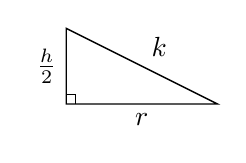
\begin{tikzpicture}[scale=0.8]
\draw[line width=0.5pt] (0,0) -- (2.4,0) -- (0,1.2) -- cycle; \draw[line width=0.4pt] (0,0.15)--(0.15,0.15)--(0.15,0);
\node[left] at (0,0.6) {$\frac{h}{2}$}; \node[below] at (1.2,0) {$r$}; \node[above right] at (1.2,0.6) {$k$};
\end{tikzpicture}}
% RVHS 2025 Promo Q1 solution diagram (conical tank with water)
\newcommand{\figRVHSsol}{\begin{tikzpicture}[scale=0.85]
\fill[blue!15] (-0.9,-1.5) -- (0,-3) -- (0.9,-1.5) arc[start angle=0,end angle=-180,x radius=0.9,y radius=0.15];
\draw[blue!50,fill=blue!8] (0,-1.5) ellipse (0.9 and 0.15);
\draw[c9] (0,0) ellipse (1.8 and 0.3); \draw[c9] (-1.8,0) -- (0,-3) -- (1.8,0);
\draw[c9aa] (0,0) -- (1.78,0); \node[above] at (0.9,0) {$3$};
\draw[c9aa] (-0.15,0) -- (-0.15,-3); \node[left] at (-0.15,-0.8) {$6$};
\draw[c9a] (0,-1.5) -- (0.88,-1.5); \node[above] at (0.45,-1.5) {$r$};
\draw[c9aa] (0.15,-1.5) -- (0.15,-3); \node[right] at (0.15,-2.2) {$h$};
\end{tikzpicture}}

\usepackage{multicol}
\usepackage{tikz-3dplot}\usepackage{colortbl}\usetikzlibrary{arrows.meta,positioning,shapes.geometric,calc}
\pgfplotsset{mini/.style={width=4.4cm,height=3.6cm,axis lines=middle,ticks=none,clip=false,xlabel=$x$,ylabel=$y$,label style={font=\small},unbounded coords=jump,every axis x label/.style={at={(ticklabel* cs:1)},anchor=west},every axis y label/.style={at={(ticklabel* cs:1)},anchor=south}},
noax/.style={width=4.8cm,height=4.4cm,axis lines=none,ticks=none,clip=false,axis equal image}}
\newcommand{\Om}{\node[anchor=north east,inner sep=1pt] at (axis cs:0,0){$O$};}
\newcommand{\ptt}[1]{\addplot[black,only marks,mark=*,mark size=1.2pt] coordinates{#1};}
\newcommand{\exg}[2]{\par\noindent\begin{minipage}[c]{0.54\textwidth}#1\end{minipage}\hspace{2mm}\begin{minipage}[c]{0.42\textwidth}\raggedright#2\end{minipage}\par\medskip}
\newcommand{\cell}[2]{\begin{minipage}[t]{0.32\textwidth}\centering#2\\[-1mm]{\small #1}\end{minipage}}

\newcommand{\vv}[1]{\mathbf{#1}}
\newcommand{\cv}[3]{\begin{pmatrix}#1\\#2\\#3\end{pmatrix}}
\newcommand{\need}[1]{{\color{blue!50!black}\textbf{Need:} #1}}
\newcommand{\sref}[1]{{\color{gray}\footnotesize\S#1}}
\newcommand{\vab}[1]{\overrightarrow{#1}}
\newcommand{\cvf}[3]{\begin{pmatrix}#1\\[1.6ex]#2\\[1.6ex]#3\end{pmatrix}}
\newcommand{\illus}{\textcolor{gray}{\footnotesize(illustration, checked)}}
\newcommand{\srcex}{}
\newcommand{\todo}[1]{\par\noindent\colorbox{yellow!30}{\parbox{\dimexpr\textwidth-2\fboxsep}{\small\textbf{DRAFT:} #1}}\par\smallskip}
\definecolor{Lcol}{RGB}{230,120,0}
%% ---- change highlighting: set \highlightfalse to switch ALL highlights off ----
\definecolor{HLc}{RGB}{255,245,120}
\newif\ifhighlight\highlighttrue
\newcommand{\hl}[1]{\ifhighlight\colorbox{HLc}{#1}\else#1\fi}
\newcommand{\hlm}[1]{\ifhighlight\colorbox{HLc}{$\displaystyle#1$}\else\ensuremath{#1}\fi}
\newcommand{\hlb}[1]{\ifhighlight\colorbox{HLc}{\parbox{\dimexpr\linewidth-2\fboxsep\relax}{\centering#1}}\else#1\fi}
\newcommand{\hlf}[1]{\ifhighlight{\setlength{\fboxrule}{1.6pt}\setlength{\fboxsep}{2pt}\fcolorbox{orange!85!yellow}{white}{#1}}\else#1\fi}
\tikzset{pt/.style={circle,fill,inner sep=1.2pt},ar/.style={-{Stealth},thick}}
\begin{document}
%% ============================================================ VECTORS I
\inchap{Vectors I}
\section{Basic Formulas}
\begin{center}\renewcommand{\arraystretch}{1.6}
\begin{tabular}{|>{\centering\arraybackslash}m{3.2cm}|>{\centering\arraybackslash}m{6.2cm}|>{\centering\arraybackslash}m{5.4cm}|}\hline
 & \textbf{Formula} & \textbf{Note}\\\Xhline{2pt}
Magnitude & $|\vv a|=\sqrt{x^{2}+y^{2}+z^{2}}$ & \\\hline
Unit vector & $\hat{\vv a}=\dfrac{\vv a}{|\vv a|}$ & $|\hat{\vv a}|=1$\\\hline
Parallel vectors & $\vv a=k\vv b$\qquad $\vv a\times\vv b=\vv 0$ & $k$ scalar constant\\\hline
Collinear $A,B,C$ & $\vab{AB}\,/\!/\,\vab{BC}$ \ (or any two of $\vab{AB},\vab{BC},\vab{AC}$) & \sidenote{Try drawing the diagram and take any two vectors, to show that they are parallel.}\\\hline
Parallelogram $ABCD$ & $\vab{AB}=\vab{DC}$,\qquad $\vab{AD}=\vab{BC}$ &
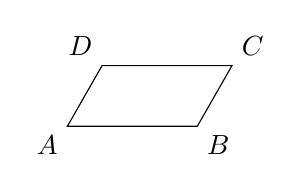
\begin{tikzpicture}[scale=0.55]\draw(0,0)node[below left]{$A$}--(3,0)node[below right]{$B$}--(3.8,1.4)node[above right]{$C$}--(0.8,1.4)node[above left]{$D$}--cycle;\end{tikzpicture}\\\hline
\end{tabular}\end{center}
\subsection*{The Ratio Theorem}
Let the points $A$, $B$ and $C$ have position vectors $\vv a$, $\vv b$ and $\vv c$ respectively, and suppose that $\lambda AC=\mu CB$. Then the position vector of $C$ is given by the formula
\begin{center}\begin{tikzpicture}[scale=0.9]
\draw(0,0)--(6,0);
\node[pt]at(0,0){};\node[below]at(0,0){$A$};\node[pt]at(6,0){};\node[below]at(6,0){$B$};\node[pt]at(2.4,0){};\node[below]at(2.4,0){$C$};
\node[pt]at(3,2.2){};\node[above]at(3,2.2){$O$};
\draw(3,2.2)--(0,0);\draw(3,2.2)--(6,0);\draw(3,2.2)--(2.4,0);
\node[below]at(1.2,-0.35){$\mu$};\node[below]at(4.2,-0.35){$\lambda$};
\end{tikzpicture}\qquad
\raisebox{8mm}{\begin{theorem}[width=4.2cm,before skip=0pt,after skip=0pt]{Ratio Theorem}\centering$\vv c=\dfrac{\lambda\vv a+\mu\vv b}{\lambda+\mu}$\end{theorem}}\end{center}
\sidenote{$AC:CB=\mu:\lambda$, so $C$ divides $AB$ with $\mu$ beside $A$ and $\lambda$ beside $B$.}\par
\sidenote{The same theorem, starting from a point $D$ instead of $O$:}
\begin{center}\begin{tikzpicture}[scale=0.9,color=gray]
\draw(0,0)--(6,0);
\node[pt]at(0,0){};\node[below]at(0,0){$A$};\node[pt]at(6,0){};\node[below]at(6,0){$B$};\node[pt]at(2.4,0){};\node[below]at(2.4,0){$C$};
\node[pt]at(3,2.2){};\node[above]at(3,2.2){$D$};
\draw(3,2.2)--(0,0);\draw(3,2.2)--(6,0);\draw(3,2.2)--(2.4,0);
\node[below]at(1.2,-0.35){$\mu$};\node[below]at(4.2,-0.35){$\lambda$};
\end{tikzpicture}\qquad
\raisebox{8mm}{\begin{theorem}[width=4.2cm,before skip=0pt,after skip=0pt,colframe=black!45,colback=black!2]{Ratio Theorem}\centering\textcolor{gray}{$\vab{DC}=\dfrac{\lambda\vab{DA}+\mu\vab{DB}}{\lambda+\mu}$}\end{theorem}}\end{center}
%% ---------------------------------------------------------------- products
\clearpage
\section{Scalar Product and Vector Product}
\topdisplay{\vv a=a_1\vv i+a_2\vv j+a_3\vv k,\qquad \vv b=b_1\vv i+b_2\vv j+b_3\vv k,\qquad\theta=\text{non-reflex }\angle AOB}
\begin{center}\renewcommand{\arraystretch}{1.25}\small
\begin{tabular}{|>{\centering\arraybackslash}m{2.4cm}|>{\centering\arraybackslash}m{6.2cm}|>{\centering\arraybackslash}m{6.2cm}|}\hline
 & \textbf{Scalar Product (Dot)} & \textbf{Vector Product (Cross)}\\\Xhline{2pt}
Definition & $\vv a\cdot\vv b=a_1b_1+a_2b_2+a_3b_3$ & $\vv a\times\vv b=\cv{a_2b_3-a_3b_2}{-(a_1b_3-a_3b_1)}{a_1b_2-a_2b_1}$\\\hline
Result & scalar & vector, $\perp$ to both $\vv a$ and $\vv b$\\\hline
Formula & $\vv a\cdot\vv b=|\vv a||\vv b|\cos\theta$ & $|\vv a\times\vv b|=|\vv a||\vv b|\sin\theta$\\\hline
Angle & $\cos\theta=\dfrac{\vv a\cdot\vv b}{|\vv a||\vv b|}$\par\sidenote{\hl{$\vv a\cdot\vv b>0$ acute, $<0$ obtuse, $=0$ right angle}} & $\sin\theta=\dfrac{|\vv a\times\vv b|}{|\vv a||\vv b|}$\par
\sidenote{this method only finds the basic angle}\par
\sidenote{possible, but usually undesirable}\\\hline
Properties &
\makecell{$\vv a\cdot\vv b=\vv b\cdot\vv a$\\ $\vv a\cdot(\vv b+\vv c)=\vv a\cdot\vv b+\vv a\cdot\vv c$\\ $\lambda(\vv a\cdot\vv b)=(\lambda\vv a)\cdot\vv b=\vv a\cdot(\lambda\vv b)$\\ $\vv a\cdot\vv a=|\vv a|^{2}$} &
\makecell{$\vv a\times\vv b=-\vv b\times\vv a$\\ $\vv a\times(\vv b+\vv c)=\vv a\times\vv b+\vv a\times\vv c$\\ $\lambda(\vv a\times\vv b)=(\lambda\vv a)\times\vv b=\vv a\times(\lambda\vv b)$\\ $\vv a\times\vv a=\vv 0$}\\\hline
Test & $\vv a\cdot\vv b=0\iff\vv a\perp\vv b$ & $\vv a\times\vv b=\vv 0\iff\vv a\,/\!/\,\vv b$\\
 & \multicolumn{2}{c|}{\sidenote{\hl{(nonzero $\vv a$, $\vv b$)}}}\\\hline
Applications &
\makecell{Length of projection $=|\vv a\cdot\hat{\vv b}|$\\ Projection vector $=(\vv a\cdot\hat{\vv b})\hat{\vv b}$} &
\makecell{Perpendicular distance $=|\vv a\times\hat{\vv b}|$\\ $\text{Area of }\triangle OAB=\tfrac12|\vv a\times\vv b|$\\ Area of parallelogram $=|\vv a\times\vv b|$}\\\hline
Geometrical meaning &
\begin{tikzpicture}[scale=0.5]
\draw[ar](0,0)--(3.4,0)node[right]{$\vv b$};\draw[ar](0,0)--(2.2,1.6)node[above]{$\vv a$};
\draw[dashed](2.2,1.6)--(2.2,0);\draw[very thick,red](0,0)--(2.2,0);\node[below,red,font=\footnotesize]at(1.1,0){$|\vv a\cdot\hat{\vv b}|$};
\end{tikzpicture}\par
$|\vv a\cdot\hat{\vv b}|$ = length of projection of $\vv a$ onto $\vv b$
&
\scriptsize\renewcommand{\arraystretch}{1}\setlength{\tabcolsep}{1.5pt}\begin{tabular}{@{}>{\centering\arraybackslash}m{1.9cm}>{\centering\arraybackslash}m{1.9cm}>{\centering\arraybackslash}m{1.9cm}@{}}
\begin{tikzpicture}[scale=0.36]
\draw[dashed](-0.6,0)--(4.4,0);
\draw[ar](0,0)--(3.2,0)node[below]{$\vv b$};\draw[ar](0,0)--(1.4,2)node[above left]{$\vv a$};
\draw[very thick,red](1.4,2)--(1.4,0);\draw(1.4,0)++(0.25,0)--++(0,0.25)--++(-0.25,0);
\node[below left]at(0,0){$O$};
\end{tikzpicture} &
\begin{tikzpicture}[scale=0.36]
\draw[fill=blue!8](0,0)--(3,0)--(4.4,2)--(1.4,2)--cycle;
\draw[ar](0,0)--(3,0)node[below]{$\vv b$};\draw[ar](0,0)--(1.4,2)node[above left]{$\vv a$};
\node[below left]at(0,0){$O$};
\end{tikzpicture} &
\begin{tikzpicture}[scale=0.36]
\draw[dashed](3,0)--(4.4,2)--(1.4,2);
\draw[fill=blue!15](0,0)--(3,0)--(1.4,2)--cycle;
\draw[ar](0,0)--(3,0)node[below]{$B$};\draw[ar](0,0)--(1.4,2)node[above left]{$A$};
\node[below left]at(0,0){$O$};
\end{tikzpicture}\\[1mm]
perpendicular distance from $A$ to line along $\vv b$\par{\color{red}$|\vv a\times\hat{\vv b}|$} &
area of parallelogram, sides $\vv a$, $\vv b$\par$|\vv a\times\vv b|$ &
$2\times$ area of $\triangle OAB$\par$|\vv a\times\vv b|$
\end{tabular}\\\hline
Note & \sidenote{$\vv a\cdot\vv b\cdot\vv c$ meaningless; no cancellation law} & \sidenote{no cancellation law}\par\sidenote{$(\vv a\times\vv b)\times\vv c$ is a vector, but triple cross products are usually not tested}\\\hline
\end{tabular}\end{center}
\begin{info}[title=Note]
Projection of $\vv a$ onto $\vv b$ $\neq$ projection of $\vv b$ onto $\vv a$. Perpendicular distance from $A$ to $OB$ $\neq$ from $B$ to $OA$. Triangles without $O$ as a vertex: $\tfrac12|\vab{AB}\times\vab{AC}|$.
\end{info}
\begin{theorem}[before skip=0pt]{Useful identity}
For any vectors $\vv a$, $\vv b$:\quad $(\vv a\times\vv b)\cdot\vv a=0$\quad and\quad $(\vv a\times\vv b)\cdot\vv b=0$\par
$\because\ \vv a\times\vv b$ is perpendicular to $\vv a$ and $\vv b$.
\end{theorem}
%% ============================================================ VECTORS II
\clearpage
\inchap{Vectors II}
\section{Equations of Lines and Planes}
\begin{center}\renewcommand{\arraystretch}{1.35}\small
\begin{tabular}{|>{\centering\arraybackslash}m{1.4cm}|>{\centering\arraybackslash}m{4.1cm}|>{\centering\arraybackslash}m{4.1cm}|>{\centering\arraybackslash}m{4.8cm}|}\hline
& \textbf{Vector} & \textbf{Cartesian} & \textbf{What you need}\\\Xhline{2pt}
\textbf{Line}&
\begin{tikzpicture}[scale=0.8]\draw[blue,thick](-0.4,-0.2)--(3,1.5);\fill(0.6,0.3)circle(1.5pt)node[below right]{$A$};\draw[-{Stealth},red,thick](0.6,0.3)--(1.8,0.9)node[above left]{$\vv b$};\fill(0,-1)circle(1.2pt)node[left]{$O$};\draw[-{Stealth}](0,-1)--(0.57,0.27)node[pos=0.5,left]{$\vv a$};\end{tikzpicture}\par
$\vv r=\vv a+\lambda\vv b,\ \lambda\in\mathbb R$\par\smallskip
$(\vv r-\vv a)\times\vv b=\vv 0$\par\sidenote{(same line: $\vv r-\vv a\,/\!/\,\vv b$)}&
\hlm{\dfrac{x-a_x}{b_x}=\dfrac{y-a_y}{b_y}=\dfrac{z-a_z}{b_z}}\par\smallskip
\sidenote{\hl{$\vv a=\left(\begin{smallmatrix}a_x\\a_y\\a_z\end{smallmatrix}\right)$, $\vv b=\left(\begin{smallmatrix}b_x\\b_y\\b_z\end{smallmatrix}\right)$}}\par\sidenote{\hl{if $b_x=0$: $x=a_x$ separately}}\par\smallskip
\sidenote{all coefficients of $x$, $y$ and $z$ in the numerators must be 1}&
\need{1 point $+$ 1 direction}\par\smallskip
or 2 points $A$, $B$:\par $\vv b=\vab{AB}$\\\hline
\textbf{Plane}&
\begin{tikzpicture}[scale=0.8]\draw[fill=blue!8](0,0)--(3,0)--(3.8,1.3)--(0.8,1.3)--cycle;\fill(1.2,0.5)circle(1.5pt)node[below]{$A$};\draw[-{Stealth},red,thick](1.2,0.5)--(2.3,0.5)node[below]{$\vv b$};\draw[-{Stealth},red,thick](1.2,0.5)--(1.65,1.1)node[right]{$\vv c$};\draw[-{Stealth},thick,green!50!black](1.2,0.5)--(1.2,1.9)node[left]{$\vv n$};\end{tikzpicture}\par
$\vv r=\vv a+\lambda\vv b+\mu\vv c$\par\smallskip
$\vv r\cdot\vv n=d$\par\sidenote{(scalar product form)}&
\hlm{n_xx+n_yy+n_zz=d}\par\sidenote{\hl{$\vv n=\left(\begin{smallmatrix}n_x\\n_y\\n_z\end{smallmatrix}\right)$}}&
\need{1 point $+$ 2 non-parallel directions $/\!/$ plane}\par\smallskip
or 1 point $+$ normal $\vv n$\par\smallskip
$\vv n=\vv b\times\vv c$,\quad $d=\vv a\cdot\vv n$\par\smallskip
\sidenote{3 points: $\vv b=\vab{AB}$, $\vv c=\vab{AC}$;\newline contains a line: use its direction}\\\hline
\end{tabular}\end{center}
\sidenote{$\vv a$: position vector of any point on the line/plane. $\vv b$, $\vv c$: any two linearly independent directions parallel to the plane. The equation of any line is not unique.}\par
\begin{info}[title=Note]
To check if a given point \hlm{C} lies on
\begin{itemize}[leftmargin=*,itemsep=1pt,topsep=1pt,parsep=0pt]
\item a line: \hlm{\vab{OC}}$=\vv a+\lambda\vv b$ \ (one $\lambda$ satisfies all 3 components)
\item a plane: \hlm{\vab{OC}}$\cdot\vv n=d$
\end{itemize}
\end{info}
\noindent\begin{minipage}[t]{0.48\textwidth}
\exlab Line through $(1,2,3)$, $(3,2,2)$ \srcex
\cdisp{\vv b&=\cv{2}{0}{-1}\\\vv r&=\cv123+\lambda\cv20{-1},\ \ \lambda\in\mathbb R\\\frac{x-1}{2}&=\frac{z-3}{-1},\quad y=2}
\end{minipage}\hfill
\begin{minipage}[t]{0.48\textwidth}
\exlab Plane through $B(0,1,1)$, $C(1,1,3)$, $D(2,0,2)$ \srcex
\cdisp{\vv n&=\vab{BC}\times\vab{BD}=\cv102\times\cv2{-1}1=\cv23{-1}\\d&=\cv011\cdot\cv23{-1}=2\\2x+3y-z&=2}
\end{minipage}
%% ---------------------------------------------------------------- map
\clearpage
\section{Interactions Map}
\begin{center}\renewcommand{\arraystretch}{1.25}\small
\begin{tabular}{|>{\centering\arraybackslash}m{1.3cm}|p{4.4cm}|p{4.4cm}|p{4.4cm}|}\hline
& \centering\textbf{Point} & \centering\textbf{Line} & \centering\arraybackslash\textbf{Plane}\\\Xhline{2pt}
\textbf{Point}& distance $|\vab{AB}|$ & \cellcolor{black!4}& \cellcolor{black!4}\\\hline
\textbf{Line}&
$\bullet$ on line? \hfill\sref{2.1}\par
$\bullet$ foot $F$ \hfill\sref{2.3}\par
$\bullet$ shortest distance \hfill\sref{2.3}\par
$\bullet$ reflection \hfill\sref{2.3}&
$\bullet$ $/\!/$ / intersect / skew \hfill\sref{2.4}\par
$\bullet$ point of intersection \hfill\sref{2.4}\par
$\bullet$ angle \hfill\sref{2.6}\par
$\bullet$ reflect line in line \hfill\sref{2.7}& \cellcolor{black!4}\\\hline
\textbf{Plane}&
$\bullet$ on plane? \hfill\sref{2.1}\par
$\bullet$ foot $F$ \hfill\sref{2.3}\par
$\bullet$ shortest distance \hfill\sref{2.3}\par
$\bullet$ reflection \hfill\sref{2.3}&
$\bullet$ $/\!/$ / lies in / intersect \hfill\sref{2.4}\par
$\bullet$ point of intersection \hfill\sref{2.4}\par
$\bullet$ angle \hfill\sref{2.6}\par
$\bullet$ reflect line in plane \hfill\sref{2.7}&
$\bullet$ $/\!/$ / same / intersect \hfill\sref{2.4}\par
$\bullet$ line of intersection \hfill\sref{2.4}\par
$\bullet$ angle \hfill\sref{2.6}\par
$\bullet$ distance ($/\!/$) \hfill\sref{2.8}\\\hline
\end{tabular}\end{center}
\sidenote{Always draw the diagram first.}
%% ---------------------------------------------------------------- card foot
\section{Foot / Distance / Reflection}
\noindent\begin{tabular}{@{}p{0.475\textwidth}|p{0.475\textwidth}@{}}
{\centering\textbf{Point $P$ -- Line $\vv r=\vv a+\lambda\vv b$}\par}\smallskip
{\centering\begin{tikzpicture}[scale=0.85]
\draw[blue,thick](-0.5,0)--(5,0)node[right]{$l$};
\fill(0.5,0)circle(1.5pt)node[below]{$A$};\draw[-{Stealth},red,thick](0.5,0)--(1.6,0)node[below]{$\vv b$};
\fill(3,1.5)circle(1.5pt)node[above]{$P$};\fill(3,0)circle(1.5pt)node[below right]{$F$};\fill(3,-1.5)circle(1.5pt)node[below]{$P'$};
\draw[dashed](3,1.5)--(3,-1.5);\draw(3,0)rectangle(3.2,0.2);\draw[densely dotted](0.5,0)--(3,1.5);
\end{tikzpicture}\par}
\begin{enumerate}[leftmargin=*,itemsep=1pt,label=\arabic*.]
\item $\vab{OF}=\vv a+\lambda\vv b$ for some $\lambda\in\mathbb R$
\item $\vab{PF}\cdot\vv b=0\ \Rightarrow$ solve for $\lambda$
\item $\vab{OF}=\dfrac{\vab{OP}+\vab{OP'}}{2}$ \ \sidenote{(midpoint / ratio theorem)}
\end{enumerate}\vspace{6mm}
&
{\centering\textbf{Point $P$ -- Plane $\vv r\cdot\vv n=d$}\par}\smallskip
{\centering\begin{tikzpicture}[scale=0.85]
\draw[fill=blue!8](0,-0.5)--(4,-0.5)--(5,0.5)--(1,0.5)--cycle;\node at(4.3,-0.25){\hlm{p}};
\fill(1.2,0)circle(1.5pt)node[below left]{$A$};
\fill(2.5,1.5)circle(1.5pt)node[above right]{$P$};\fill(2.5,0)circle(1.5pt)node[below right]{$F$};\fill(2.5,-1.5)circle(1.5pt)node[below]{$P'$};
\draw[dashed](2.5,1.5)--(2.5,-1.5);\draw[densely dotted](1.2,0)--(2.5,1.5);\draw[-{Stealth},green!50!black,thick](1.2,0)--(1.2,1)node[left]{$\vv n$};
\end{tikzpicture}\par}
\begin{enumerate}[leftmargin=*,itemsep=1pt,label=\arabic*.]
\item $l_{PF}:\ \vv r=\hlm{\vab{OP}}+\lambda\vv n$,\ $\lambda\in\mathbb R$
\item $(\hlm{\vab{OP}}+\lambda\vv n)\cdot\vv n=d$ \sidenote{(intersection between line \& plane)} $\Rightarrow$ solve for $\lambda$
\item $\vab{OF}=\dfrac{\vab{OP}+\vab{OP'}}{2}$ \ \sidenote{(midpoint / ratio theorem)}
\end{enumerate}\vspace{6mm}
\\
\begin{theorem}[before skip=2mm,after skip=2mm]{Distance}
\centering$PF=|\vab{AP}\times\hat{\vv b}|$
\end{theorem}
&
\begin{theorem}[before skip=2mm,after skip=2mm]{Distance}
\centering$PF=|\vab{AP}\cdot\hat{\vv n}|$
\end{theorem}
\end{tabular}\par\medskip
\noindent\begin{tabular}{@{}p{0.475\textwidth}|p{0.475\textwidth}@{}}
{\centering\textbf{Reflection (and foot of perpendicular) of point to line}\par}\smallskip
&
{\centering\textbf{Reflection (and foot of perpendicular) of point to plane}\par}\smallskip
\\
\raggedright\exlab Find the foot of the perpendicular $N$ from $A(3,-2,-1)$ to the line $l_1$, and the reflection $A'$ of $A$ in $l_1$, where\par\noindent\hfill$l_1:\ \vv r=\cv123+\lambda\cv30{-1},\ \ \lambda\in\mathbb R$\hfill\null\par
\begin{center}\begin{tikzpicture}[scale=0.72]
\draw[blue,thick](-0.5,0)--(5.2,0)node[right,font=\footnotesize]{$l_1$};
\fill(3,2.2)circle(1.5pt)node[above,font=\footnotesize]{$A(3,-2,-1)$};\fill(3,0)circle(1.5pt)node[below right,font=\footnotesize]{$N(4,2,2)$};\fill(3,-2.2)circle(1.5pt)node[below,font=\footnotesize]{$A'(5,6,5)$};
\draw[dashed](3,2.2)--(3,-2.2);\draw(3,0)rectangle(3.25,0.25);
\end{tikzpicture}\end{center}
\cdisp{\vab{AN}&=\cv{-2+3\lambda}{4}{4-\lambda}\\
\vab{AN}\cdot\cv30{-1}&=0\\10\lambda-10&=0\ \Rightarrow\ \lambda=1\\
\therefore\ N&=(4,2,2)\\
\vab{ON}&=\dfrac{\vab{OA}+\vab{OA'}}{2}\ \ \text{\sidenote{(midpoint/ratio theorem)}}\\
\Rightarrow\ \vab{OA'}&=2\vab{ON}-\vab{OA}\\
\vab{OA'}&=2\cv422-\cv3{-2}{-1}\\\therefore\ A'&=(5,6,5)}
&
\raggedright\exlab Find the foot of the perpendicular $F$ from $P(7,0,3)$ to the plane $p$, and the reflection $P'$ of $P$ in $p$, where\par\noindent\hfill$p:\ \vv r\cdot\cv112=1$\hfill\null\par
\begin{center}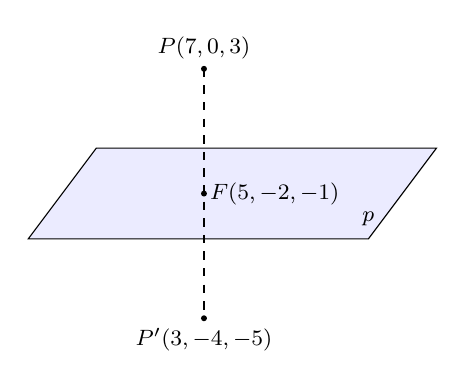
\begin{tikzpicture}[scale=0.72]
\draw[fill=blue!8](0,-0.8)--(6,-0.8)--(7.2,0.8)--(1.2,0.8)--cycle;\node[font=\footnotesize]at(6.0,-0.45){$p$};
\fill(3.1,2.2)circle(1.5pt)node[above,font=\footnotesize]{$P(7,0,3)$};\fill(3.1,0)circle(1.5pt)node[right,xshift=1pt,fill=blue!8,inner sep=1pt,font=\footnotesize]{$F(5,-2,-1)$};\fill(3.1,-2.2)circle(1.5pt)node[below,font=\footnotesize]{$P'(3,-4,-5)$};
\draw[dashed](3.1,2.2)--(3.1,-2.2);
\end{tikzpicture}\end{center}
\cdisp{\hlm{l_{PF}:\ \vv r}&=\hlm{\cv703+\lambda\cv112,\ \ \lambda\in\mathbb R}\\\left(\cv703+\lambda\cv112\right)\cdot\cv112&=1\\13+6\lambda&=1\ \Rightarrow\ \lambda=-2\\
\therefore\ F&=(5,-2,-1)\\
\vab{OF}&=\dfrac{\vab{OP}+\vab{OP'}}{2}\ \ \text{\sidenote{(midpoint/ratio theorem)}}\\
\Rightarrow\ \vab{OP'}&=2\vab{OF}-\vab{OP}\\
\vab{OP'}&=2\cv5{-2}{-1}-\cv703\\\therefore\ P'&=(3,-4,-5)}
\end{tabular}
\clearpage
\noindent\begin{tabular}{@{}p{0.475\textwidth}|p{0.475\textwidth}@{}}
{\centering\textbf{Shortest distance from point to line}\par}\smallskip
&
{\centering\textbf{Shortest distance from point to plane}\par}\smallskip
\\
\raggedright\exlab Find the shortest distance from $P(5,1,3)$ to the line\par\noindent\hfill$l:\ \vv r=\cv102+\lambda\cv2{-1}2,\ \ \lambda\in\mathbb R$\hfill\null\par
\begin{center}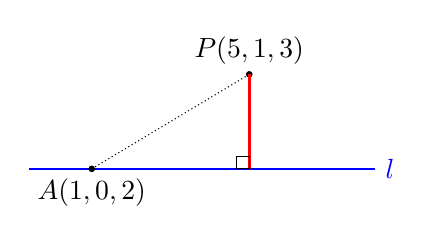
\begin{tikzpicture}[scale=0.8]
\draw[blue,thick](-0.5,0)--(5,0)node[right]{$l$};
\fill(0.5,0)circle(1.5pt)node[below]{$A(1,0,2)$};
\fill(3,1.5)circle(1.5pt)node[above]{$P(5,1,3)$};
\draw[densely dotted](0.5,0)--(3,1.5);\draw[very thick,red](3,1.5)--(3,0);\draw(3,0)rectangle(2.8,0.2);
\end{tikzpicture}\end{center}
\cdisp{\text{shortest distance}&=|\vab{AP}\times\hat{\vv b}|\\
&=\left|\cv411\times\frac13\cv2{-1}2\right|\\
&=\left|\frac13\cv3{-6}{-6}\right|=\left|\cv1{-2}{-2}\right|\\
&=3}
&
\raggedright\exlab Find the shortest distance from $P(4,4,1)$ to the plane\par\noindent\hfill$p:\ \vv r\cdot\cv21{-2}=4$\hfill\null\par
\begin{center}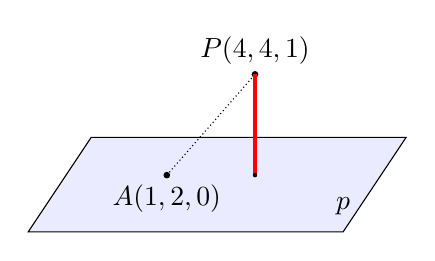
\begin{tikzpicture}[scale=0.8]
\draw[fill=blue!8](0,-0.9)--(5,-0.9)--(6,0.6)--(1,0.6)--cycle;\node at(5.0,-0.5){$p$};
\fill(2.2,0)circle(1.5pt)node[below]{$A(1,2,0)$};
\fill(3.6,1.6)circle(1.5pt)node[above]{$P(4,4,1)$};
\draw[densely dotted](2.2,0)--(3.6,1.6);\draw[very thick,red](3.6,1.6)--(3.6,0);\fill(3.6,0)circle(1pt);
\end{tikzpicture}\end{center}
\cdisp{\text{shortest distance}&=|\vab{AP}\cdot\hat{\vv n}|\\
&=\left|\cv321\cdot\frac13\cv21{-2}\right|\\
&=\left|\frac13(6+2-2)\right|\\
&=2}
\end{tabular}\par\medskip
\begin{info}[title=Note]
We can also find the coordinates of the foot of the perpendicular $N$ first, then take $|\vab{PN}|$, but this is less efficient.
\end{info}
%% ---------------------------------------------------------------- relationships
\clearpage
\section{Relationships and Intersections}
\tikzset{q/.style={diamond,draw,aspect=2.6,fill=black!5,inner sep=1pt,align=center,font=\small},
r/.style={rectangle,rounded corners,draw,thick,fill=blue!8,minimum width=2.5cm,minimum height=0.75cm,align=center,font=\small},
qb/.style={rectangle,draw,fill=black!5,inner sep=4pt,text width=5.3cm,align=center,font=\small}}
\subsection*{Line -- Line \quad $l_1:\vv r=\vv a_1+\lambda\hlm{\vv b_1}$,\ \ $l_2:\vv r=\vv a_2+\mu\hlm{\vv b_2}$}
\begin{center}\renewcommand{\arraystretch}{1.3}\small
\begin{tabular}{|>{\centering\arraybackslash}m{1.6cm}|>{\centering\arraybackslash}m{4.3cm}|>{\centering\arraybackslash}m{4.3cm}|>{\centering\arraybackslash}m{4.3cm}|}\hline
 & \textbf{Parallel} & \textbf{Intersecting} & \textbf{Skew}\\\Xhline{2pt}
\textbf{Diagram} &
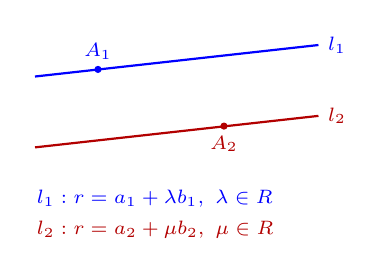
\begin{tikzpicture}[scale=1]
\draw[blue,thick](0,1.1)--(3.6,1.5);\draw[red!70!black,thick](0,0.2)--(3.6,0.6);
\fill[blue](0.8,1.19)circle(1.3pt)node[above,font=\scriptsize]{$A_1$};\fill[red!70!black](2.4,0.47)circle(1.3pt)node[below,font=\scriptsize]{$A_2$};
\node[blue,font=\scriptsize,right]at(3.6,1.5){$l_1$};\node[red!70!black,font=\scriptsize,right]at(3.6,0.6){$l_2$};
\node[anchor=west,font=\scriptsize,text=blue] at(-0.1,-0.45){$l_1:\vv r=\vv a_1+\lambda\vv b_1,\ \lambda\in\mathbb R$};
\node[anchor=west,font=\scriptsize,text=red!70!black] at(-0.1,-0.85){$l_2:\vv r=\vv a_2+\mu\vv b_2,\ \mu\in\mathbb R$};
\end{tikzpicture}&
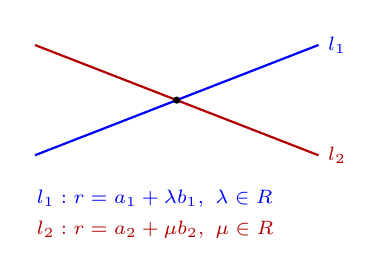
\begin{tikzpicture}[scale=1]
\draw[blue,thick](0,0.1)--(3.6,1.5);\draw[red!70!black,thick](0,1.5)--(3.6,0.1);
\fill(1.8,0.8)circle(1.3pt);
\node[blue,font=\scriptsize,right]at(3.6,1.5){$l_1$};\node[red!70!black,font=\scriptsize,right]at(3.6,0.1){$l_2$};
\node[anchor=west,font=\scriptsize,text=blue] at(-0.1,-0.45){$l_1:\vv r=\vv a_1+\lambda\vv b_1,\ \lambda\in\mathbb R$};
\node[anchor=west,font=\scriptsize,text=red!70!black] at(-0.1,-0.85){$l_2:\vv r=\vv a_2+\mu\vv b_2,\ \mu\in\mathbb R$};
\end{tikzpicture}&
\hlf{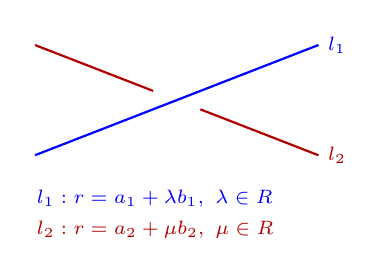
\begin{tikzpicture}[scale=1]
\draw[red!70!black,thick](0,1.5)--(1.5,0.917);\draw[red!70!black,thick](2.1,0.683)--(3.6,0.1);
\draw[blue,thick](0,0.1)--(3.6,1.5);
\node[blue,font=\scriptsize,right]at(3.6,1.5){$l_1$};\node[red!70!black,font=\scriptsize,right]at(3.6,0.1){$l_2$};
\node[anchor=west,font=\scriptsize,text=blue] at(-0.1,-0.45){$l_1:\vv r=\vv a_1+\lambda\vv b_1,\ \lambda\in\mathbb R$};
\node[anchor=west,font=\scriptsize,text=red!70!black] at(-0.1,-0.85){$l_2:\vv r=\vv a_2+\mu\vv b_2,\ \mu\in\mathbb R$};
\end{tikzpicture}}\\\hline
\textbf{Condition} & \hlb{$\vv b_1\,/\!/\,\vv b_2$ and $A_1\notin l_2$, $A_2\notin l_1$} & \hlb{$\vv b_1\nparallel \vv b_2$, unique solution for $\lambda$ and $\mu$} & \hlb{$\vv b_1\nparallel \vv b_2$, no solution for $\lambda$ and $\mu$}\\\hline
\end{tabular}\end{center}
\begin{center}\begin{tikzpicture}
\node[qb,text width=4.2cm](q1) at(0,0){Is $l_1$ parallel to $l_2$?\\[-1pt]\sidenote{i.e. \hlm{\vv b_1=k\vv b_2}?}};
\node[qb](qa) at(-3.5,-2.4){Does point $A_1$ lie on $l_2$ or point $A_2$ lie on $l_1$?};
\node[qb](qb2) at(3.5,-2.4){Does $\vv a_1+\lambda\vv b_1=\vv a_2+\mu\vv b_2$ have a unique solution for $\lambda$ and $\mu$?};
\node[r](s1) at(-5.1,-4.6){same line};\node[r](s2) at(-1.9,-4.6){parallel};
\node[r](s3) at(1.9,-4.6){intersecting};\node[r](s4) at(5.1,-4.6){skew};
\draw[ar](q1.south)--node[above left,font=\footnotesize,pos=0.55]{yes}(qa.north);
\draw[ar](q1.south)--node[above right,font=\footnotesize,pos=0.55]{no}(qb2.north);
\draw[ar](qa.south)--node[above left,font=\footnotesize,pos=0.55]{yes}(s1.north);
\draw[ar](qa.south)--node[above right,font=\footnotesize,pos=0.55]{no}(s2.north);
\draw[ar](qb2.south)--node[above left,font=\footnotesize,pos=0.55]{yes}(s3.north);
\draw[ar](qb2.south)--node[above right,font=\footnotesize,pos=0.55]{no}(s4.north);
\end{tikzpicture}\end{center}
\begin{info}[title=Note]
Definition of \textbf{skew lines}:
\begin{itemize}[leftmargin=*,itemsep=0pt,topsep=1pt,parsep=0pt]
\item non parallel
\item non intersecting
\end{itemize}
Thus, to prove that two lines are skew, we must first state that \hlm{\vv b_1\neq k\vv b_2}, so $l_1$ and $l_2$ are not parallel, before proceeding with simultaneous equations to show they have no solution.
\end{info}
\clearpage
\exlab Determine whether $l_1$ and $l_2$ are intersecting or skew lines.\par
\noindent\hfill$l_1:\ \vv r=\cv102+\lambda\cv121,\ \ \lambda\in\mathbb R$\hfill\null\par
\noindent\hfill$l_2:\ \vv r=\cv2{12}5+\mu\cv{-1}30,\ \ \mu\in\mathbb R$\hfill\null\par
\cdisp{1+\lambda&=2-\mu\lb1\\2\lambda&=12+3\mu\lb2\\2+\lambda&=5\lb3\\
\text{From (1) and (3), }\lambda&=3,\ \ \mu=-2\\
\text{Sub into (2), LHS}&=6,\ \ \text{RHS}=12+3(-2)=6\\
\therefore\ \text{LHS}&=\text{RHS}\\
\text{Sub }\lambda=3\text{ into }l_1:\ \vv r&=\cv102+3\cv121=\cv465\\
\text{They intersect at}\ &(4,6,5)}
\sidenote{Solve 2 of the 3 equations, sub into the 3rd: LHS $=$ RHS $\Rightarrow$ intersect; LHS $\neq$ RHS $\Rightarrow$ skew.}
\clearpage
\subsection*{Line -- Plane \quad $l:\vv r=\vv a+\lambda\vv b$,\ \ $\hlm{p}:\vv r\cdot\vv n=d$}\label{sec:lineplane}
\begin{center}\renewcommand{\arraystretch}{1.3}\small
\begin{tabular}{|>{\centering\arraybackslash}m{1.6cm}|>{\centering\arraybackslash}m{4.3cm}|>{\centering\arraybackslash}m{4.3cm}|>{\centering\arraybackslash}m{4.3cm}|}\hline
 & \textbf{Parallel, not on the plane} & \textbf{Line lies in the plane} & \textbf{Intersects at one point}\\\Xhline{2pt}
\textbf{Diagram} &
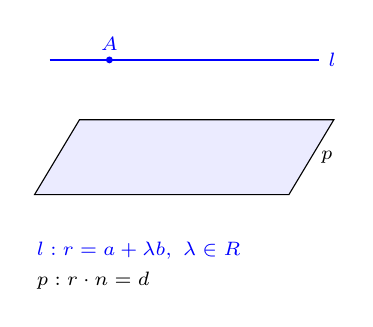
\begin{tikzpicture}[scale=0.95]
\draw[fill=blue!8](0,0)--(3.4,0)--(4.0,1.0)--(0.6,1.0)--cycle;\node[font=\scriptsize,right]at(3.7,0.5){$p$};
\draw[blue,thick](0.2,1.8)--(3.8,1.8);\fill[blue](1.0,1.8)circle(1.3pt)node[above,font=\scriptsize]{$A$};\node[blue,font=\scriptsize,right]at(3.8,1.8){$l$};
\node[anchor=west,font=\scriptsize,text=blue] at(-0.1,-0.75){$l:\vv r=\vv a+\lambda\vv b,\ \lambda\in\mathbb R$};
\node[anchor=west,font=\scriptsize,text=black] at(-0.1,-1.15){$p:\vv r\cdot\vv n=d$};
\end{tikzpicture}&
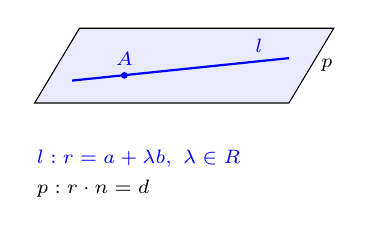
\begin{tikzpicture}[scale=0.95]
\draw[fill=blue!8](0,0)--(3.4,0)--(4.0,1.0)--(0.6,1.0)--cycle;\node[font=\scriptsize,right]at(3.7,0.5){$p$};
\draw[blue,thick](0.5,0.3)--(3.4,0.6);\fill[blue](1.2,0.37)circle(1.3pt)node[above,font=\scriptsize]{$A$};\node[blue,font=\scriptsize,above]at(3.0,0.55){$l$};
\node[anchor=west,font=\scriptsize,text=blue] at(-0.1,-0.75){$l:\vv r=\vv a+\lambda\vv b,\ \lambda\in\mathbb R$};
\node[anchor=west,font=\scriptsize,text=black] at(-0.1,-1.15){$p:\vv r\cdot\vv n=d$};
\end{tikzpicture}&
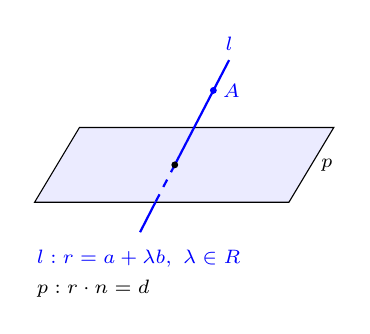
\begin{tikzpicture}[scale=0.95]
\draw[fill=blue!8](0,0)--(3.4,0)--(4.0,1.0)--(0.6,1.0)--cycle;\node[font=\scriptsize,right]at(3.7,0.5){$p$};
\draw[blue,thick](2.6,1.9)--(1.874,0.5);\draw[blue,thick,dashed](1.874,0.5)--(1.615,0);\draw[blue,thick](1.615,0)--(1.41,-0.4);\fill[blue](2.39,1.495)circle(1.3pt)node[right,font=\scriptsize]{$A$};\fill(1.874,0.5)circle(1.3pt);\node[blue,font=\scriptsize,above]at(2.6,1.9){$l$};
\node[anchor=west,font=\scriptsize,text=blue] at(-0.1,-0.75){$l:\vv r=\vv a+\lambda\vv b,\ \lambda\in\mathbb R$};
\node[anchor=west,font=\scriptsize,text=black] at(-0.1,-1.15){$p:\vv r\cdot\vv n=d$};
\end{tikzpicture}\\\hline
\textbf{Condition} & \footnotesize$\bullet$ normal $\perp$ line: $\vv b\cdot\vv n=0$\par $\bullet$ $A$ does not lie on $p$: $\vv a\cdot\vv n\neq d$ & \footnotesize$\bullet$ normal $\perp$ line: $\vv b\cdot\vv n=0$\par $\bullet$ $A$ lies on $p$: $\vv a\cdot\vv n=d$ & \footnotesize$\bullet$ normal not $\perp$ line: $\vv b\cdot\vv n\neq0$\\\hline
\end{tabular}\end{center}
\begin{center}\begin{tikzpicture}
\node[qb,text width=4.2cm](q1) at(0,0){Normal of plane $\perp$ line?\\[-1pt]\sidenote{$\vv b\cdot\vv n=0$?}};
\node[qb,text width=4.2cm](qa) at(-3.5,-2.4){Does $A$ lie on $p$?\\[-1pt]\sidenote{$\vv a\cdot\vv n=d$?}};
\node[r](s3) at(3.5,-2.4){intersect at one point};
\node[r](s1) at(-5.3,-4.6){line lies in plane};\node[r](s2) at(-1.7,-4.6){parallel, not on the plane};
\draw[ar](q1.south)--node[above left,font=\footnotesize,pos=0.55]{yes}(qa.north);
\draw[ar](q1.south)--node[above right,font=\footnotesize,pos=0.55]{no}(s3.north);
\draw[ar](qa.south)--node[above left,font=\footnotesize,pos=0.55]{yes}(s1.north);
\draw[ar](qa.south)--node[above right,font=\footnotesize,pos=0.55]{no}(s2.north);
\end{tikzpicture}\end{center}
\exlab Find the point of intersection between the line $l$ and plane $p$.\par
\noindent\hfill$l:\ \vv r=\cv131+\lambda\cv1{-2}1,\ \ \lambda\in\mathbb R$\hfill\null\par
\noindent\hfill$p:\ \vv r\cdot\cv121=5$\hfill\null\par
\cdisp{\vv r&=\cv131+\lambda\cv1{-2}1=\cv{1+\lambda}{3-2\lambda}{1+\lambda},\ \ \lambda\in\mathbb R\\
\cv{1+\lambda}{3-2\lambda}{1+\lambda}\cdot\cv121&=5\\8-2\lambda&=5\ \Rightarrow\ \lambda=\tfrac32\\\therefore\ &(2.5,0,2.5)}
\clearpage
\subsection*{Plane -- Plane \quad $p_1:\vv r\cdot\vv n_1=d_1$,\ \ $p_2:\vv r\cdot\vv n_2=d_2$}
\noindent\hl{Let $p_1:\ \vv r\cdot\vv n_1=d_1$ and $p_2:\ \vv r\cdot\vv n_2=d_2$ be distinct planes.}\par\smallskip
\begin{center}\renewcommand{\arraystretch}{1.3}\small
\begin{tabular}{|>{\centering\arraybackslash}m{1.6cm}|>{\centering\arraybackslash}m{4.3cm}|>{\centering\arraybackslash}m{4.3cm}|}\hline
 & \textbf{Parallel} & \textbf{Intersecting in a line}\\\Xhline{2pt}
\textbf{Diagram} &
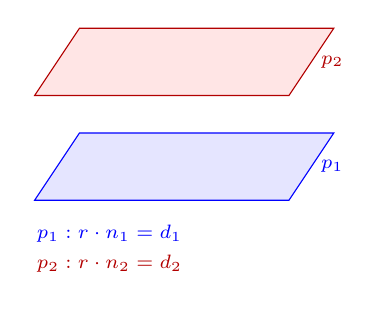
\begin{tikzpicture}[scale=0.95]
\draw[fill=blue!10,draw=blue](0,0)--(3.4,0)--(4.0,0.9)--(0.6,0.9)--cycle;\node[blue,font=\scriptsize,right]at(3.7,0.45){$p_1$};
\draw[fill=red!10,draw=red!70!black](0,1.4)--(3.4,1.4)--(4.0,2.3)--(0.6,2.3)--cycle;\node[red!70!black,font=\scriptsize,right]at(3.7,1.85){$p_2$};
\node[anchor=west,font=\scriptsize,text=blue] at(-0.1,-0.45){$p_1:\vv r\cdot\vv n_1=d_1$};
\node[anchor=west,font=\scriptsize,text=red!70!black] at(-0.1,-0.85){$p_2:\vv r\cdot\vv n_2=d_2$};
\end{tikzpicture}&
\begin{tikzpicture}[x={(1.0cm,0cm)},y={(0.5cm,0.35cm)},z={(0cm,0.9cm)}]
\filldraw[fill=blue,fill opacity=0.4,draw=blue!60!black,line width=0.5pt](-1.2,-1,0)--(-1.2,1,0)--(1.2,1,0)--(1.2,-1,0)--cycle;
\filldraw[fill=red,fill opacity=0.4,draw=red!60!black,line width=0.5pt](-0.5,-1,-1)--(0.5,-1,1)--(0.5,1,1)--(-0.5,1,-1)--cycle;
\node[blue!60!black,font=\scriptsize,right]at(1.2,1,0){$p_1$};\node[red!60!black,font=\scriptsize,above]at(0.5,1,1){$p_2$};
\draw[Lcol,line width=3pt,line cap=round](0,-1.15,0)--(0,1.15,0);
\node[anchor=west,font=\scriptsize,text=blue] at(-1.7cm,-1.6cm){$p_1:\vv r\cdot\vv n_1=d_1$};
\node[anchor=west,font=\scriptsize,text=red!70!black] at(-1.7cm,-2.0cm){$p_2:\vv r\cdot\vv n_2=d_2$};
\end{tikzpicture}\\\hline
\textbf{Condition} & $\vv n_1\,/\!/\,\vv n_2$, $p_1\neq p_2$ & $\vv n_1\nparallel \vv n_2$\\\hline
\end{tabular}\end{center}
\begin{center}\begin{tikzpicture}
\node[qb,text width=4.2cm](q1) at(0,0){Is $p_1$ parallel to $p_2$?\\[-1pt]\sidenote{i.e. $\vv n_1=k\vv n_2$?}};
\node[qb,text width=4.8cm](qa) at(-3.5,-2.4){Does a point on $p_1$ lie on $p_2$?\\[-1pt]\sidenote{i.e. \hlm{d_1=kd_2}?}\\[-1pt]\sidenote{\hl{(same $k$ as $\vv n_1=k\vv n_2$)}}};
\node[r,align=center](s3) at(3.5,-2.4){intersect in a line\\[-1pt]\footnotesize direction $\vv n_1\times\vv n_2$};
\node[r](s1) at(-5.1,-4.6){same plane};\node[r](s2) at(-1.9,-4.6){parallel};
\draw[ar](q1.south)--node[above left,font=\footnotesize,pos=0.55]{yes}(qa.north);
\draw[ar](q1.south)--node[above right,font=\footnotesize,pos=0.55]{no}(s3.north);
\draw[ar](qa.south)--node[above left,font=\footnotesize,pos=0.55]{yes}(s1.north);
\draw[ar](qa.south)--node[above right,font=\footnotesize,pos=0.55]{no}(s2.north);
\end{tikzpicture}\end{center}
\exlab Find the intersection between the planes:\par\noindent\hfill$\begin{aligned}3x+2y+z&=10\\x-2y+z&=5\end{aligned}$\hfill\null\par
\cdisp{\text{GC:}\ x&=\dfrac{15}{4}-\dfrac12z\\
y&=-\dfrac58+\dfrac14z\\
z&=z\\
\therefore\ l:\ \vv r&=\cvf{\dfrac{15}{4}}{-\dfrac58}{0}+\lambda\cvf{-\dfrac12}{\dfrac14}{1},\ \ \lambda\in\mathbb R}
\providecolor{Lcol}{RGB}{230,120,0}
\clearpage
\exlab Sometimes, we may not be able to use our GC to find the line of intersection between two planes. The steps to find it manually are:\par\noindent\hfill$p_1:\ \vv r\cdot\cv111=6$,\qquad $p_2:\ \vv r\cdot\cv1{-1}2=2$\hfill\null\par
\noindent\begin{minipage}[c]{0.5\textwidth}\raggedright
\textbf{Step 1:} direction $=\vv n_1\times\vv n_2$
\cdisp{\hlm{\vv b}&=\cv111\times\cv1{-1}2\\
&=\cv{1(2)-1(-1)}{1(1)-1(2)}{1(-1)-1(1)}\\
&=\cv3{-1}{-2}}
\end{minipage}\hfill
\begin{minipage}[c]{0.46\textwidth}\centering
\begin{tikzpicture}[x={(1.5cm,0cm)},y={(0.8cm,0.55cm)},z={(0cm,1.35cm)}]
\filldraw[fill=blue,fill opacity=0.4,draw=blue!60!black,line width=0.5pt](-1.2,-1,0)--(-1.2,1,0)--(1.2,1,0)--(1.2,-1,0)--cycle;
\filldraw[fill=red,fill opacity=0.4,draw=red!60!black,line width=0.5pt](-0.5,-1,-1)--(0.5,-1,1)--(0.5,1,1)--(-0.5,1,-1)--cycle;
\node[blue!60!black,font=\scriptsize,right]at(1.2,1,0){$p_1$};\node[red!60!black,font=\scriptsize,above]at(0.5,1,1){$p_2$};
\draw[Lcol,line width=2.4pt,line cap=round,-{Stealth[length=3mm]}](0,-1,0)--(0,1.3,0)node[right,font=\scriptsize,text=Lcol]{$\vv n_1\times\vv n_2$};
\draw[blue!60!black,thick,-{Stealth}](-0.9,-0.3,0)--(-0.9,-0.3,1.2)node[above,font=\scriptsize]{$\vv n_1$};
\draw[red!60!black,thick,-{Stealth}](-0.3,-0.3,-0.6)--(0.7,-0.3,-1.1)node[below right,font=\scriptsize]{$\vv n_2$};
\end{tikzpicture}
\end{minipage}\par\medskip
\textbf{Step 2:} find a point that lies on both planes
\cdisp{p_1:\ x+y+z&=6\\
p_2:\ x-y+2z&=2\\
\text{Let }z&=0}
\sys{x+y&=6\\x-y&=2}{\begin{aligned}x&=4\\y&=2\end{aligned}}
\cdisp{\therefore\ l:\ \vv r&=\cv420+\lambda\cv3{-1}{-2},\ \ \lambda\in\mathbb R}
\tikzset{pv/.style={x={(1.15cm,0cm)},y={(0.6cm,0.42cm)},z={(0cm,1.05cm)},baseline=(current bounding box.center)}}
\definecolor{Lcol}{RGB}{230,120,0}
\newcommand{\Pq}[5]{\filldraw[fill=#1,fill opacity=0.4,draw=#1!60!black,line width=0.5pt](#2)--(#3)--(#4)--(#5)--cycle;}
\newcommand{\Pg}[4]{\filldraw[fill=black!12,fill opacity=0.55,draw=black!35,line width=0.4pt](#1)--(#2)--(#3)--(#4)--cycle;}
\newcommand{\Ln}[2]{\draw[Lcol,line width=2.4pt,line cap=round](#1)--(#2);}
\clearpage
\section{Interaction between 3 Planes}
\tikzset{pvs/.style={x={(0.8cm,0cm)},y={(0.42cm,0.29cm)},z={(0cm,0.74cm)},baseline=(current bounding box.center)}}
\renewcommand{\Ln}[2]{\draw[Lcol,line width=1.8pt,line cap=round](#1)--(#2);}
\newcommand{\lcond}{\textcolor{Lcol}{$l:\ \vv r=\vv a+\lambda\vv b,\ \lambda\in\mathbb R$}}
\newcommand{\pthree}{\textcolor{green!55!black}{$p_3$}}
\newcommand{\arr}{\raisebox{0pt}{$\Rightarrow$}}
\noindent\hl{Let $p_1:\ \vv r\cdot\vv n_1=d_1$, $p_2:\ \vv r\cdot\vv n_2=d_2$ and $p_3:\ \vv r\cdot\vv n_3=d_3$ be distinct planes.}\par\smallskip
\begin{center}\renewcommand{\arraystretch}{1.45}\small\setlength{\tabcolsep}{4pt}
\begin{tabular}{|>{\centering\arraybackslash}m{2.5cm}|>{\centering\arraybackslash}m{8.3cm}|>{\centering\arraybackslash}m{4.6cm}|}\hline
\textbf{Case} & \textbf{Diagram(s)} & \textbf{Condition}\par\hlb{\footnotesize\textcolor{Lcol}{$l$}: line of intersection of $p_1$ and $p_2$ ($\vv n_1\nparallel\vv n_2$)}\\\Xhline{2pt}
\textbf{1. All parallel} &
\begin{tikzpicture}[pvs]
\Pq{blue}{-1.2,-1,-1}{-1.2,1,-1}{1.2,1,-1}{1.2,-1,-1}
\Pq{red}{-1.2,-1,0}{-1.2,1,0}{1.2,1,0}{1.2,-1,0}
\Pq{green!55!black}{-1.2,-1,1}{-1.2,1,1}{1.2,1,1}{1.2,-1,1}
\node[blue!60!black,font=\scriptsize,right]at(1.2,1,-1){$p_1$};
\node[red!60!black,font=\scriptsize,right]at(1.2,1,0){$p_2$};
\node[green!55!black,font=\scriptsize,right]at(1.2,1,1){$p_3$};
\end{tikzpicture} & \footnotesize$\vv n_1\parallel\vv n_2\parallel\vv n_3$\\\hline
\textbf{2. Two parallel, one not} &
\begin{tikzpicture}[pvs]
\Pq{blue}{-1.2,-1,-0.7}{-1.2,1,-0.7}{1.2,1,-0.7}{1.2,-1,-0.7}
\Pq{red}{-1.2,-1,0.7}{-1.2,1,0.7}{1.2,1,0.7}{1.2,-1,0.7}
\Pq{green!55!black}{-1.3,-0.2,-1.3}{1.3,-0.2,-1.3}{1.3,0.2,1.3}{-1.3,0.2,1.3}
\draw[black,line width=0.9pt](-1.2,-0.1077,-0.7)--(1.2,-0.1077,-0.7);
\draw[black,line width=0.9pt](-1.2,0.1077,0.7)--(1.2,0.1077,0.7);
\node[blue!60!black,font=\scriptsize,right]at(1.2,1,-0.7){$p_1$};
\node[red!60!black,font=\scriptsize,right]at(1.2,1,0.7){$p_2$};
\node[green!55!black,font=\scriptsize,above right]at(1.3,0.2,1.3){$p_3$};
\end{tikzpicture} & \footnotesize$\vv n_1\parallel\vv n_2$, but $\vv n_3$ not parallel to them\\\hline
\textbf{3. All intersect at 1 point}\par\sidenote{(most common)} &
\begin{tikzpicture}[pvs]
\Pq{blue}{-1.2,-1,0}{-1.2,1,0}{1.2,1,0}{1.2,-1,0}
\Pq{red}{-0.5,-1,-1}{0.5,-1,1}{0.5,1,1}{-0.5,1,-1}
\Ln{0,-1,0}{0,1,0}
\node[blue!60!black,font=\scriptsize,right]at(1.2,1,0){$p_1$};
\node[red!60!black,font=\scriptsize,above]at(0.5,1,1){$p_2$};
\end{tikzpicture}\ \raisebox{0pt}{\large$\Rightarrow$}\ 
\begin{tikzpicture}[pvs]
\Pg{-1.2,-1,0}{-1.2,1,0}{1.2,1,0}{1.2,-1,0}
\Pg{-0.5,-1,-1}{0.5,-1,1}{0.5,1,1}{-0.5,1,-1}
\Pq{green!55!black}{-1.2,-0.26,-1}{1.2,0.46,-1}{1.2,0.86,1}{-1.2,0.14,1}
\draw[black!45,dashed,line width=0.9pt](-1.2,-0.06,0)--(1.2,0.66,0);
\draw[black!45,dashed,line width=0.9pt](-0.5,-0.05,-1)--(0.5,0.65,1);
\Ln{0,-1,0}{0,1,0}
\filldraw[fill=black,draw=white,line width=0.6pt](0,0.3,0)circle(2pt);
\node[green!55!black,font=\scriptsize,above left]at(-1.2,0.14,1){$p_3$};
\end{tikzpicture} &
\footnotesize\lcond\par intersects \pthree\par (see p.~\pageref{sec:lineplane})\\\hline
\textbf{4. All intersect in a line} &
\begin{tikzpicture}[pvs]
\Pq{blue}{-1.2,-1,0}{-1.2,1,0}{1.2,1,0}{1.2,-1,0}
\Pq{red}{-0.5,-1,-1}{0.5,-1,1}{0.5,1,1}{-0.5,1,-1}
\Ln{0,-1,0}{0,1,0}
\node[blue!60!black,font=\scriptsize,right]at(1.2,1,0){$p_1$};
\node[red!60!black,font=\scriptsize,above]at(0.5,1,1){$p_2$};
\end{tikzpicture}\ \raisebox{0pt}{\large$\Rightarrow$}\ 
\begin{tikzpicture}[pvs]
\Pg{-1.2,-1,0}{-1.2,1,0}{1.2,1,0}{1.2,-1,0}
\Pg{-0.5,-1,-1}{0.5,-1,1}{0.5,1,1}{-0.5,1,-1}
\Pq{green!55!black}{-1,-1,0.9}{-1,1,0.9}{1,1,-0.9}{1,-1,-0.9}
\Ln{0,-1,0}{0,1,0}
\node[green!55!black,font=\scriptsize,right]at(1,1,-0.9){$p_3$};
\end{tikzpicture} &
\footnotesize\lcond\par lies on \pthree\par (see p.~\pageref{sec:lineplane})\\\hline
\textbf{5. Form a triangular prism}\par\sidenote{(no single point of intersection)} &
\begin{tikzpicture}[pvs]
\Pq{blue}{-0.6,-1,0}{-0.6,1,0}{1.3,1,0}{1.3,-1,0}
\Pq{red}{-0.25,-1,-0.5}{0.65,-1,1.3}{0.65,1,1.3}{-0.25,1,-0.5}
\Ln{0,-1,0}{0,1,0}
\node[blue!60!black,font=\scriptsize,right]at(1.3,1,0){$p_1$};
\node[red!60!black,font=\scriptsize,above]at(0.65,1,1.3){$p_2$};
\end{tikzpicture}\ \raisebox{0pt}{\large$\Rightarrow$}\ 
\begin{tikzpicture}[pvs]
\Pg{-0.6,-1,0}{-0.6,1,0}{1.3,1,0}{1.3,-1,0}
\Pg{-0.25,-1,-0.5}{0.65,-1,1.3}{0.65,1,1.3}{-0.25,1,-0.5}
\Pq{green!55!black}{0.69,-1,-0.3}{0.69,1,-0.3}{0.21,1,1.3}{0.21,-1,1.3}
\draw[black!45,dashed,line width=0.9pt](0.6,-1,0)--(0.6,1,0);
\draw[black!45,dashed,line width=0.9pt](0.375,-1,0.75)--(0.375,1,0.75);
\Ln{0,-1,0}{0,1,0}
\node[green!55!black,font=\scriptsize,above]at(0.21,1,1.3){$p_3$};
\end{tikzpicture} &
\hlb{\footnotesize\lcond\par $\bullet$ \textcolor{Lcol}{$l\,/\!/\,$}\pthree: $\vv b\cdot\vv n_3=0$\par $\bullet$ \textcolor{Lcol}{$l\not\subset$}\pthree: $\vv a\cdot\vv n_3\neq d_3$\par (see p.~\pageref{sec:lineplane})}\\\hline
\end{tabular}\end{center}
\begin{info}[title=Note]
To analyse the interaction between 3 arbitrary planes, we can study how the \textcolor{Lcol}{\textbf{line of intersection between $p_1$ and $p_2$}} interacts with \textcolor{green!55!black}{$p_3$}.
\end{info}
%% angles
\section{Angles}
\begin{center}\renewcommand{\arraystretch}{1.5}
\begin{tabular}{|>{\centering\arraybackslash}m{4.6cm}|>{\centering\arraybackslash}m{4.6cm}|>{\centering\arraybackslash}m{4.6cm}|}\hline
\textbf{Line -- Line} & \textbf{Line -- Plane} & \textbf{Plane -- Plane}\\\Xhline{2pt}
\begin{tikzpicture}[scale=0.75]\draw[blue,thick](0,0)--(3,1.2);\draw[red,thick](0,1.2)--(3,0);\draw(1.95,0.78)arc(22:-22:0.5);\node[font=\footnotesize]at(2.3,0.6){$\theta$};\node[font=\footnotesize,above]at(3,1.2){\hlm{\vv b_1}};\node[font=\footnotesize,below]at(3,0){\hlm{\vv b_2}};\end{tikzpicture}&
\begin{tikzpicture}[scale=0.75]\draw[fill=blue!8](0,0)--(3,0)--(3.6,0.8)--(0.6,0.8)--cycle;\draw[red,thick](1,0.4)--(3,1.8)node[right,font=\footnotesize]{$\vv b$};\draw[dashed](1,0.4)--(3,0.4);\draw[dashed](3,0.4)--(3,1.8);\draw[green!50!black,ar](1,0.4)--(1,1.8)node[left,font=\footnotesize]{$\vv n$};\draw(1.5,0.4)arc(0:35:0.5);\node[font=\footnotesize]at(1.75,0.6){$\theta$};\end{tikzpicture}&
\begin{tikzpicture}[x={(0.95cm,0cm)},y={(0.5cm,0.35cm)},z={(0cm,0.9cm)},baseline=(current bounding box.center)]
\Pq{blue}{-1.2,-1,0}{-1.2,1,0}{1.2,1,0}{1.2,-1,0}
\Pq{red}{-0.5,-1,-1}{0.5,-1,1}{0.5,1,1}{-0.5,1,-1}
\Ln{0,-1,0}{0,1,0}
\draw[black,line width=0.5pt](0.45,-1,0)arc[start angle=0,end angle=63.4,x radius=0.45*0.95cm,y radius=0.45*0.9cm];
\node[font=\scriptsize]at(0.78,-1,0.14){$\theta$};
\node[blue!60!black,font=\scriptsize,right]at(1.2,1,0){$p_1$};
\node[red!60!black,font=\scriptsize,above]at(0.5,1,1){$p_2$};
\end{tikzpicture}\\
\hlm{\cos\theta=\dfrac{|\vv b_1\cdot\vv b_2|}{|\vv b_1||\vv b_2|}} &
$\sin\theta=\left|\dfrac{\vv n\cdot\vv b}{|\vv n||\vv b|}\right|$ &
$\cos\theta=\left|\dfrac{\vv n_1\cdot\vv n_2}{|\vv n_1||\vv n_2|}\right|$\\
\sidenote{directions} & \sidenote{$\sin$: $\angle(\vv n,\vv b)=90^\circ-\theta$} & \sidenote{normals}\\\hline
\end{tabular}\end{center}
\sidenote{$\theta$ = acute angle.}\par
\sidenote{Each formula has a modulus in the numerator $\because$ $\theta$ must be acute.}\par
\noindent\begin{minipage}[t]{0.48\textwidth}
\exlab Find the angle between the planes $3x-y+2z=3$ and $y=2$.\par
\cdisp{\cos\theta&=\frac{|-1|}{\sqrt{14}\cdot1}\\\theta&=74.5^\circ}
\end{minipage}\hfill
\begin{minipage}[t]{0.48\textwidth}
\exlab Find the angle between the line $l$ and plane $p$.\par
\noindent\hfill$l:\ \vv r=\cv{-2}{-4}5+\lambda\cv35{-4},\ \ \lambda\in\mathbb R$\hfill\null\par
\noindent\hfill$p:\ \vv r\cdot\cv010=1$\hfill\null\par
\cdisp{\sin\theta&=\frac{5}{\sqrt{50}\cdot1}=\frac1{\sqrt2}\\\theta&=45^\circ}
\end{minipage}
%% ---------------------------------------------------------------- reflection of lines
\section{Reflection of a Line}
\noindent\begin{minipage}[t]{0.48\textwidth}
\centering\textbf{Line $l_1$ in line $l_2$} \sidenote{(intersect at $X$)}\par\smallskip
\begin{tikzpicture}[scale=0.8]
\draw[blue,thick](-0.3,0)--(5,0)node[right]{$l_2$};
\draw[red,thick](0.5,0)--(3.6,1.6)node[above]{$l_1$};\draw[red,thick,dashed](0.5,0)--(3.6,-1.6)node[below]{$l_1'$};
\fill(0.5,0)circle(1.5pt)node[below left]{$X$};
\fill(3,1.29)circle(1.5pt)node[above left]{$A$};\fill(3,0)circle(1.5pt)node[below right]{$F$};\fill(3,-1.29)circle(1.5pt)node[below left]{$A'$};
\draw[densely dotted](3,1.29)--(3,-1.29);
\node[anchor=west,font=\scriptsize,text=red] at(-0.3,-2.2){$l_1:\vv r=\vv a_1+\lambda\vv b_1,\ \lambda\in\mathbb R$};
\node[anchor=west,font=\scriptsize,text=blue] at(-0.3,-2.7){$l_2:\vv r=\vv a_2+\mu\vv b_2,\ \mu\in\mathbb R$};
\end{tikzpicture}
\begin{enumerate}[leftmargin=*,itemsep=1pt,label=\arabic*.]
\item $X=l_1\cap l_2$
\item $A\in l_1$: foot $F$ on $l_2$
\item $\vab{OF}=\dfrac{\vab{OA}+\vab{OA'}}{2}$ \sidenote{(midpoint/ratio theorem)}
\item $l_1':\ \vv r=\vab{OX}+\mu\vab{XA'},\ \mu\in\mathbb R$
\end{enumerate}
\end{minipage}\hfill
\begin{minipage}[t]{0.48\textwidth}
\centering\textbf{Line $l$ in plane $p$} \sidenote{(intersect at $X$)}\par\smallskip
\begin{tikzpicture}[scale=0.8]
\draw[fill=blue!8](0,-0.5)--(4,-0.5)--(5,0.5)--(1,0.5)--cycle;\node at(4.4,-0.25){$p$};
\draw[red,thick](1.5,0)--(3.5,1.8)node[above]{$l$};\draw[red,thick,dashed](1.5,0)--(3.5,-1.8)node[below]{$l'$};
\fill(1.5,0)circle(1.5pt)node[left]{$X$};
\fill(3,1.35)circle(1.5pt)node[right]{$A$};\fill(3,0)circle(1.5pt)node[below right]{$F$};\fill(3,-1.35)circle(1.5pt)node[right]{$A'$};
\draw[densely dotted](3,1.35)--(3,-1.35);
\node[anchor=west,font=\scriptsize,text=red] at(0,-2.2){$l:\vv r=\vv a+\lambda\vv b,\ \lambda\in\mathbb R$};
\node[anchor=west,font=\scriptsize,text=black] at(0,-2.7){$p:\vv r\cdot\vv n=d$};
\end{tikzpicture}
\begin{enumerate}[leftmargin=*,itemsep=1pt,label=\arabic*.]
\item $X=l\cap p$
\item $A\in l$: foot $F$ on $p$
\item $\vab{OF}=\dfrac{\vab{OA}+\vab{OA'}}{2}$ \sidenote{(midpoint/ratio theorem)}
\item $l':\ \vv r=\vab{OX}+\mu\vab{XA'},\ \mu\in\mathbb R$
\end{enumerate}
\end{minipage}\par\smallskip
\sidenote{If $l\,/\!/\,p$: $l'$ has the same direction, through $A'$.}\par
%% ---------------------------------------------------------------- distance
\section{Distance Between Parallel Planes}
\noindent\begin{minipage}[c]{0.55\textwidth}
\topdisplay{p:\ \vv r\cdot\vv n=d}
\begin{theorem}[before skip=2mm,after skip=2mm]{Distance of plane from origin}
\centering$\text{distance from }O=\dfrac{|d|}{|\vv n|}$
\end{theorem}
\end{minipage}\hfill
\begin{minipage}[c]{0.4\textwidth}\centering
\begin{tikzpicture}[scale=0.8]
\draw[fill=blue!8](0.2,1.4)--(3.6,1.4)--(4.4,2.2)--(1.0,2.2)--cycle;\node[right] at(4.4,2.0){$p$};
\fill(1.6,0)circle(1.5pt)node[below]{$O$};
\fill(1.6,1.8)circle(1.5pt)node[below left,font=\footnotesize]{$N$};
\draw[densely dashed](1.6,0)--(1.6,1.8);
\draw(1.6,1.55)--(1.85,1.55)--(1.85,1.8);
\node[left,font=\footnotesize]at(1.55,0.8){$\dfrac{|d|}{|\vv n|}$};
\draw[green!50!black,ar](1.6,1.8)--(1.6,2.7)node[above,font=\footnotesize]{$\vv n$};
\end{tikzpicture}\end{minipage}\par\medskip
\noindent\begin{minipage}[c]{0.55\textwidth}
\topdisplay{p_1:\ \vv r\cdot\vv n=d_1,\qquad p_2:\ \vv r\cdot\vv n=d_2}
\begin{theorem}[before skip=2mm,after skip=2mm]{Distance}
\centering$\text{distance}=\left|\dfrac{d_1}{|\vv n|}-\dfrac{d_2}{|\vv n|}\right|$
\end{theorem}
\sidenote{Same $\vv n$ for both planes first. $\vv r\cdot\vv n=0$: plane through $O$.}
\end{minipage}\hfill
\begin{minipage}[c]{0.4\textwidth}\centering
\begin{tikzpicture}[scale=0.8]
\draw[fill=blue!8](0,1.6)--(3.4,1.6)--(4.2,2.3)--(0.8,2.3)--cycle;\node[right] at(4.2,2.1){$p_1$};
\draw[fill=blue!8](0,0)--(3.4,0)--(4.2,0.7)--(0.8,0.7)--cycle;\node[right] at(4.2,0.5){$p_2$};
\draw[<->,thick](2,0.35)--(2,1.95);\node[right,font=\footnotesize]at(2,1.15){distance};
\end{tikzpicture}\end{minipage}
\exlab Find the distance between the two planes $x+2y-3z=2$ and $2x+4y-6z=-10$.\par
\cdisp{2x+4y-6z&=-10\ \Rightarrow\ x+2y-3z=-5\\
\text{distance}&=\left|\frac{2}{\sqrt{14}}-\frac{-5}{\sqrt{14}}\right|=\frac{7}{\sqrt{14}}=\hlm{\frac{\sqrt{14}}{2}}}
\end{document}
